\chapter{Diagramme der Auswertung}
In diesem Kapitel finden Sie Diagramme der Auswertungen zu den im Methodologieteil gestellten Fragen. Einzelne, aus unserer Sicht, relevante Diagramme sind hier nicht aufgef�hrt, da diese direkt im Kapitel <<Ergebnisse / Resultate>> abgebildet wurden.

\begin{figure}[h]
	\centering
		
	\ifpdf
		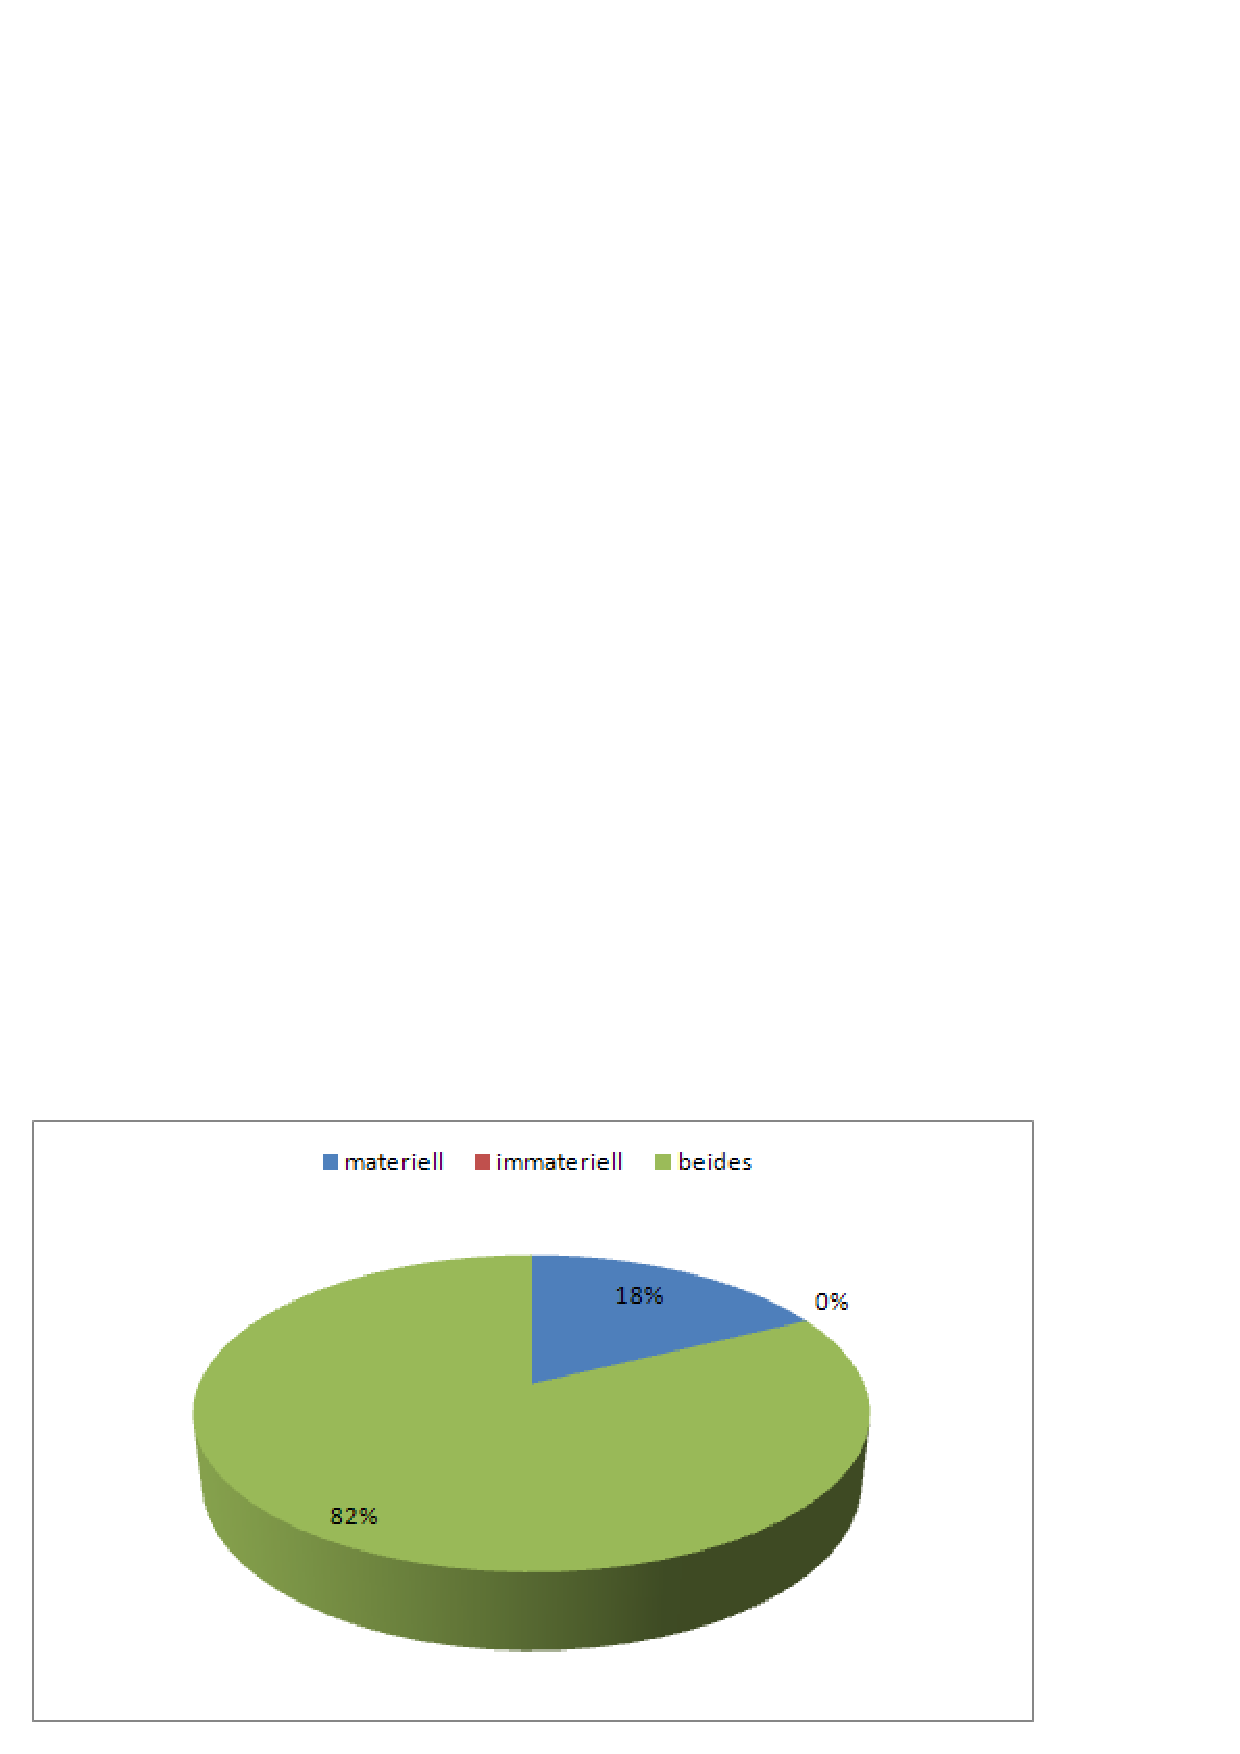
\includegraphics[width=0.9\textwidth]{chap12-unternehmen-anreizmix.png}
	\else	
		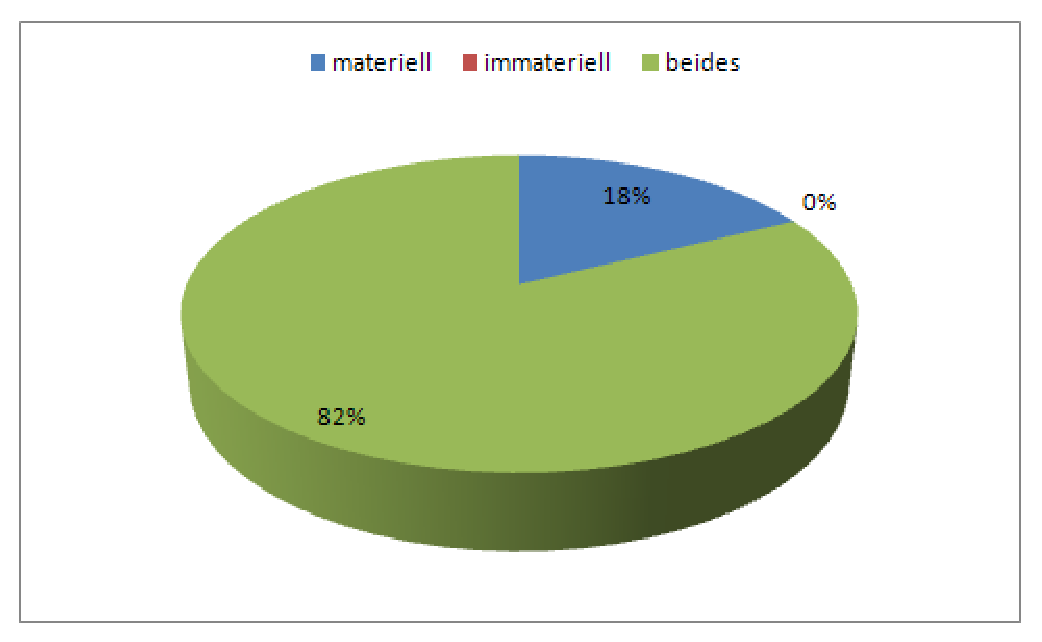
\includegraphics[width=0.9\textwidth]{chap12-unternehmen-anreizmix.eps}
	\fi
		
	\caption[Anreizmix aus Sicht von Unternehmen]{Anreizmix aus Sicht von Unternehmen (eigene Darstellung)}	
	\label{fig:anreizMixUnternehmen}
\end{figure}

\begin{figure}[h]
	\centering
		
	\ifpdf
		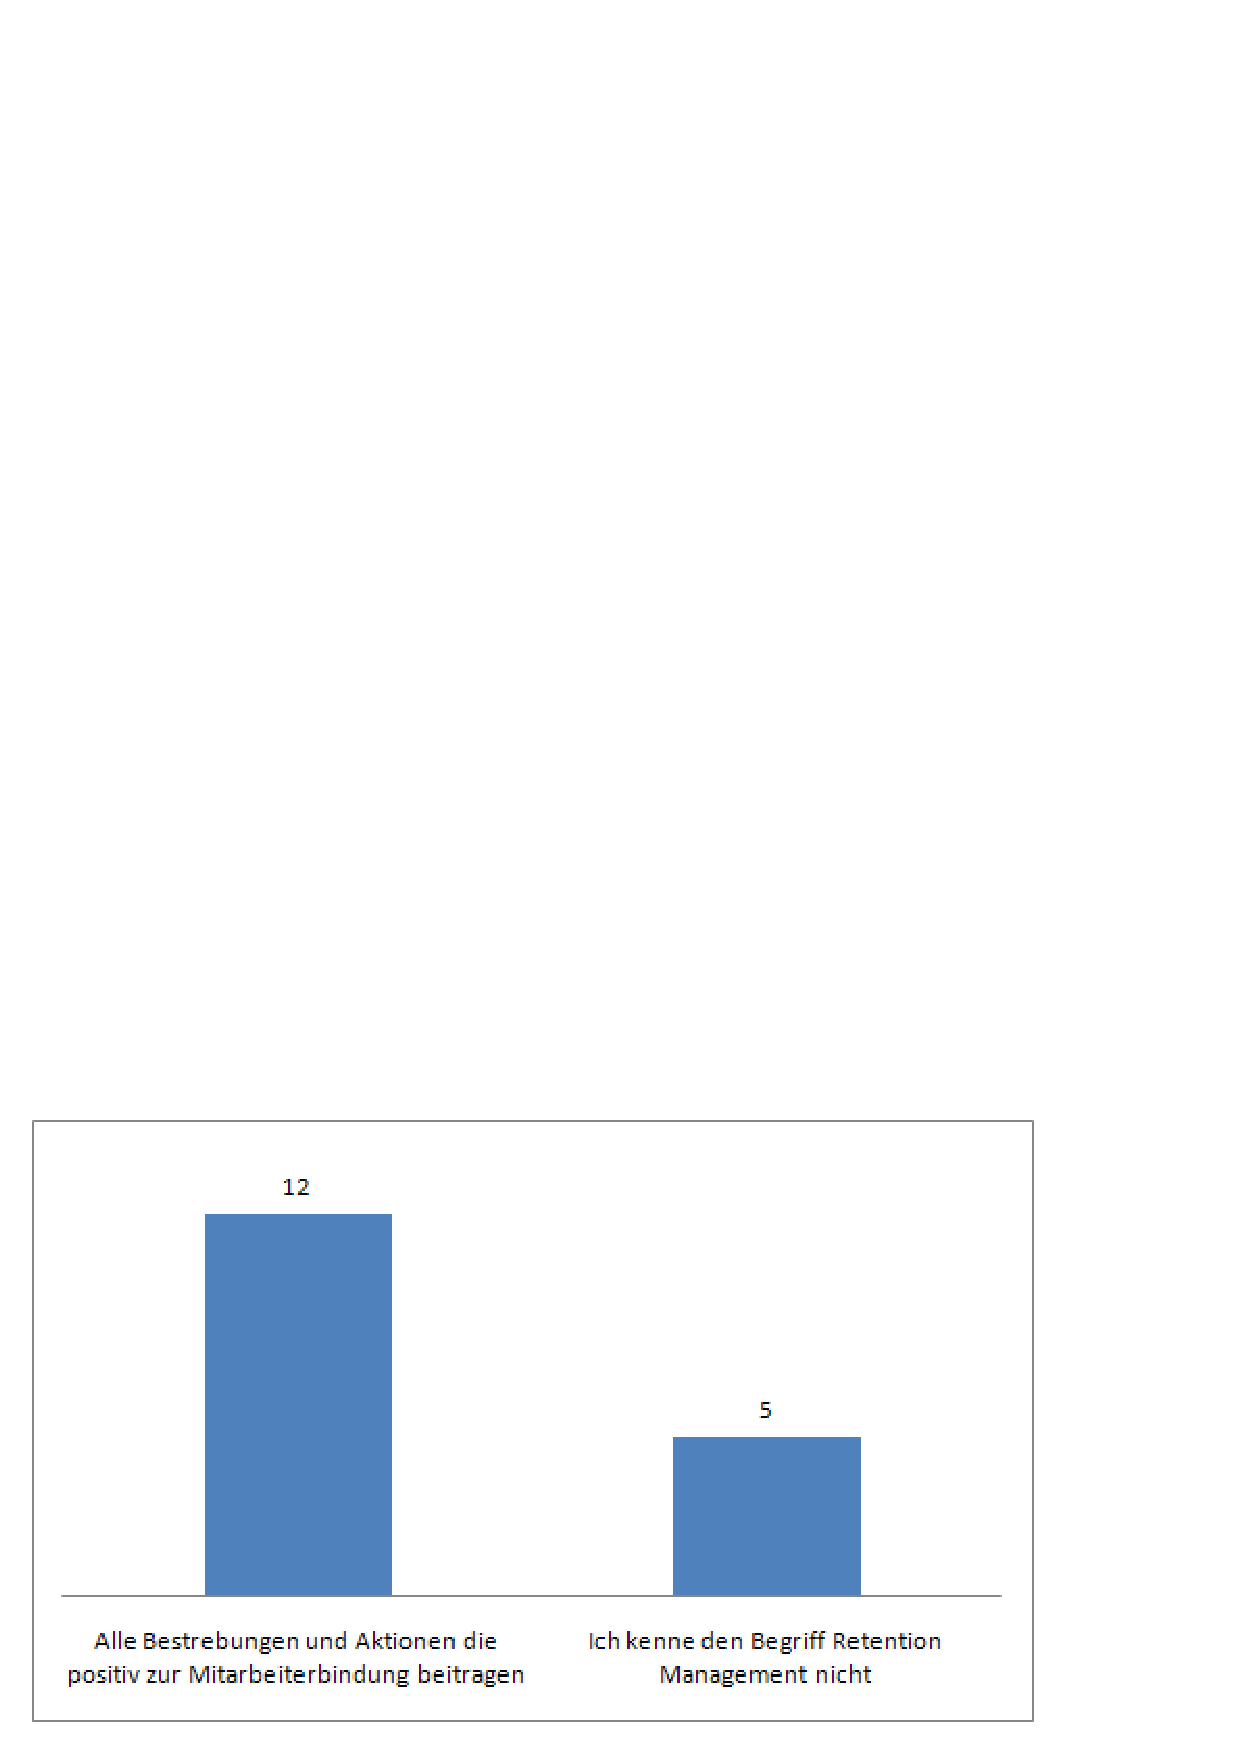
\includegraphics[width=0.9\textwidth]{chap12-unternehmen-retentionmanagement.png}
	\else	
		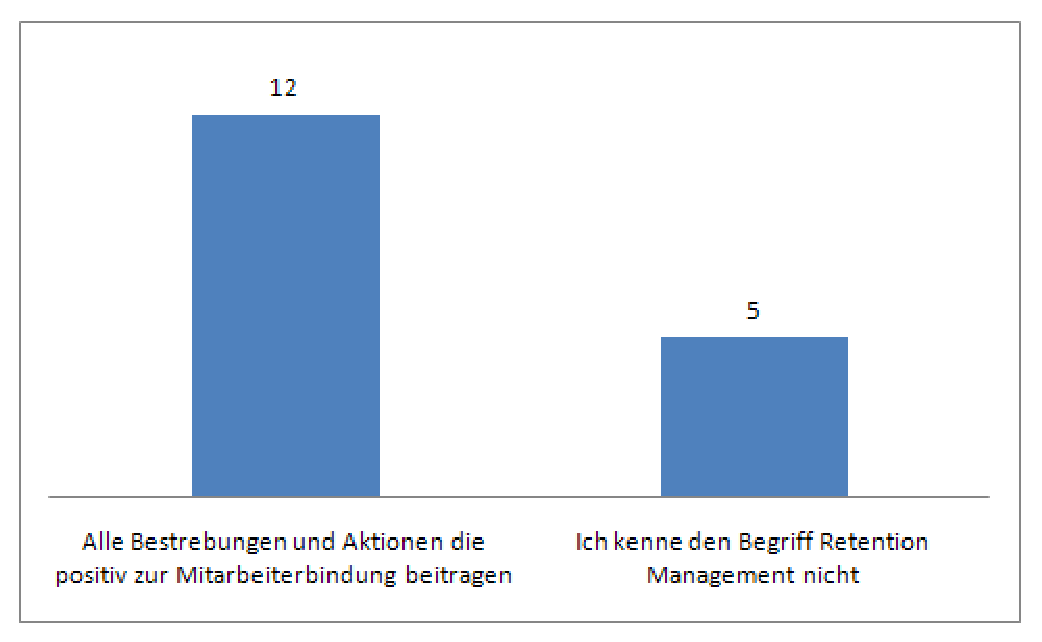
\includegraphics[width=0.9\textwidth]{chap12-unternehmen-retentionmanagement.eps}
	\fi
		
	\caption[Verst�ndnis von Retention Management]{Verst�ndnis von Retention Management (eigene Darstellung)}	
	\label{fig:whatIsRetention}
\end{figure}

\begin{figure}[h]
	\centering
		
	\ifpdf
		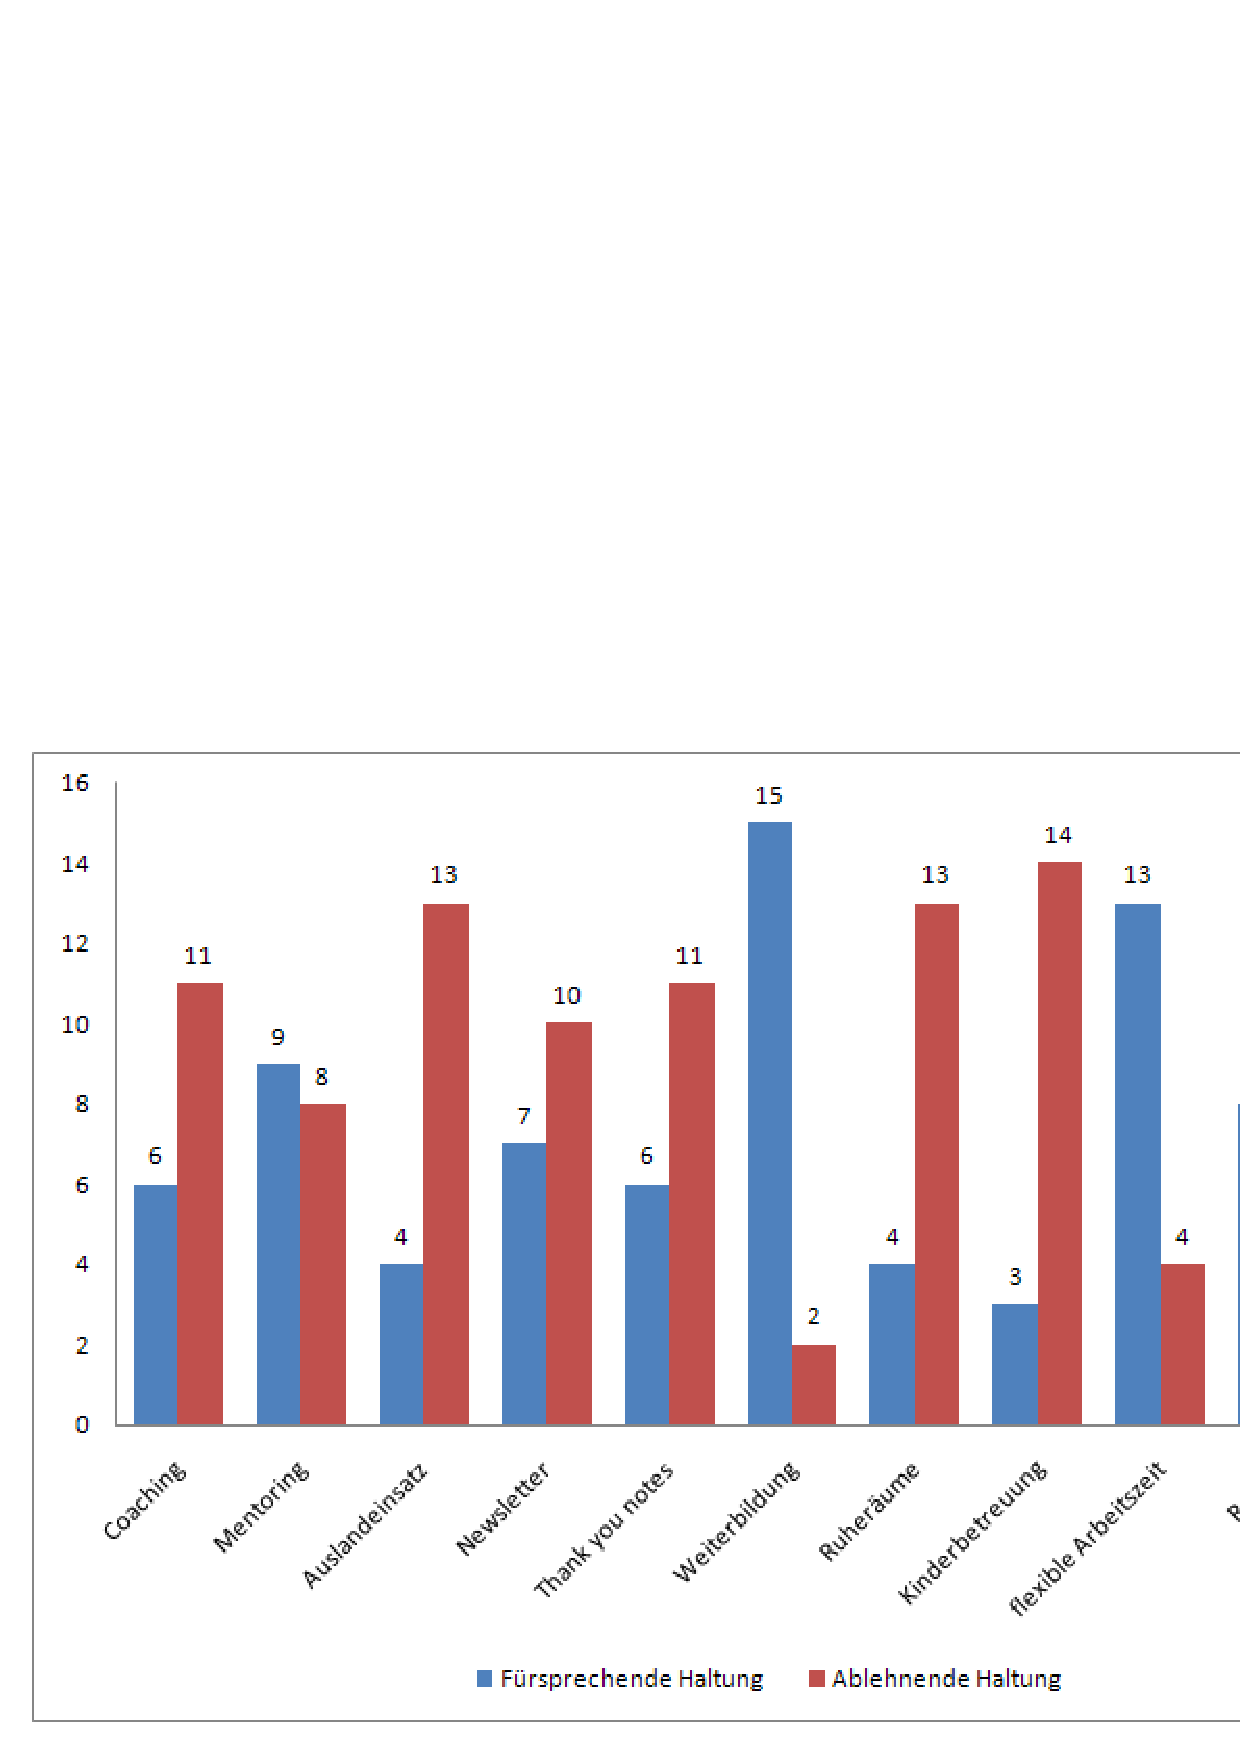
\includegraphics[width=0.9\textwidth]{chap12-unternehmen-proUndContra.png}
	\else	
		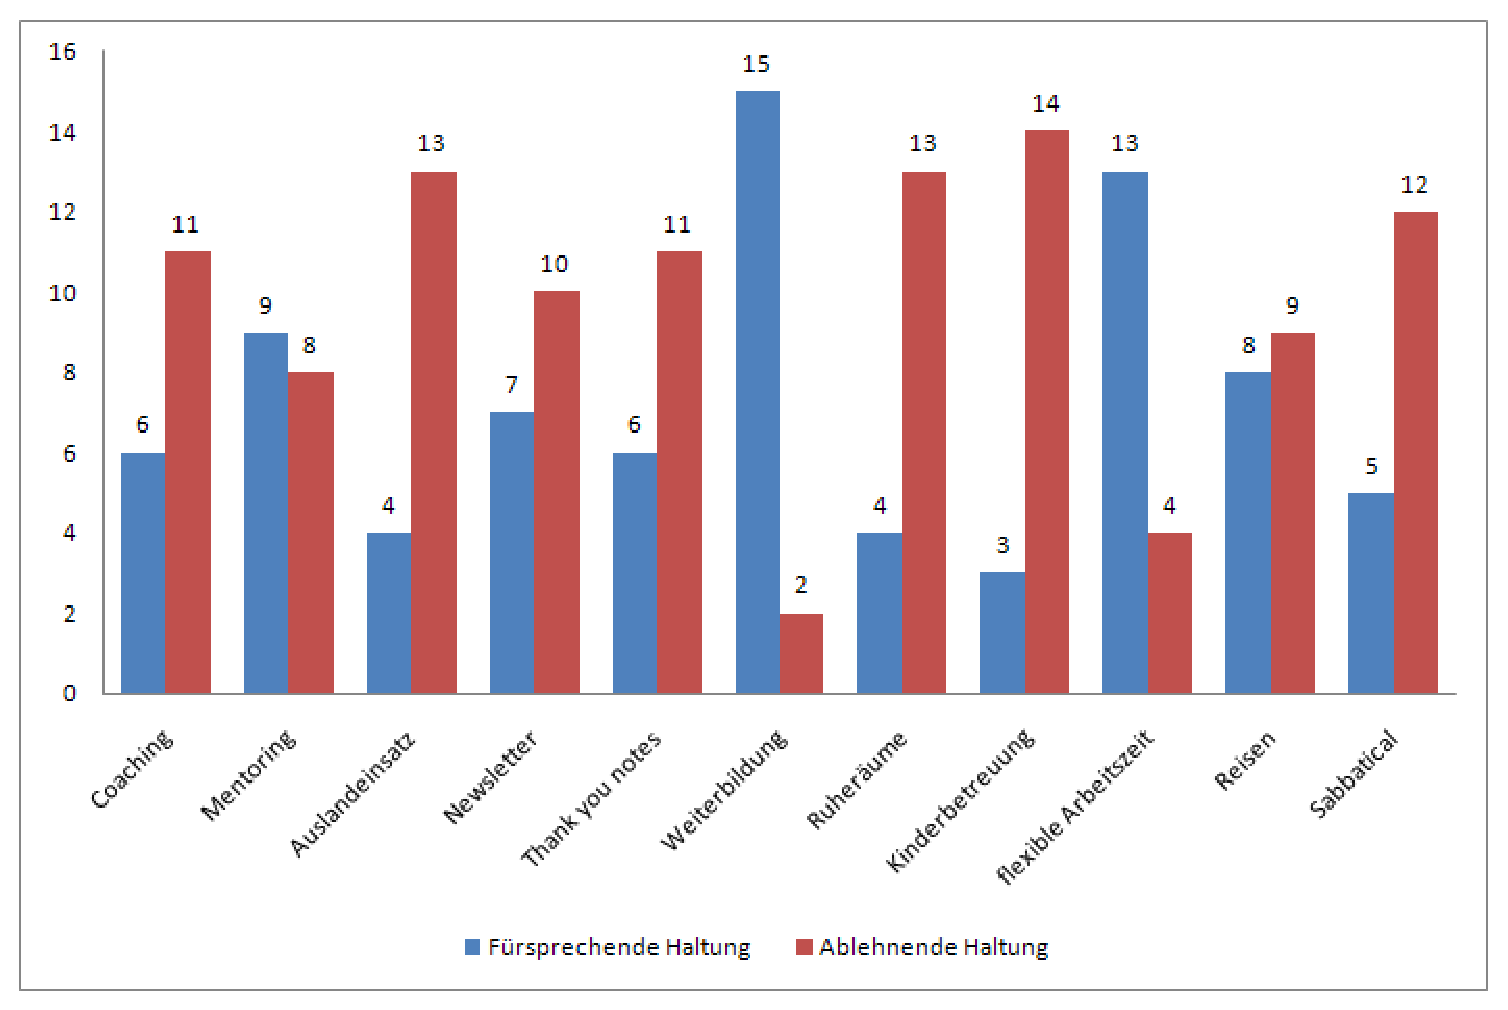
\includegraphics[width=0.9\textwidth]{chap12-unternehmen-proUndContra.eps}
	\fi
		
	\caption[Haltungen zu immaterielle Anreizen]{Haltungen zu immaterielle Anreizen (eigene Darstellung)}	
	\label{fig:anreizHaltungUnternehmen}
\end{figure}

\begin{figure}[h]
	\centering
		
	\ifpdf
		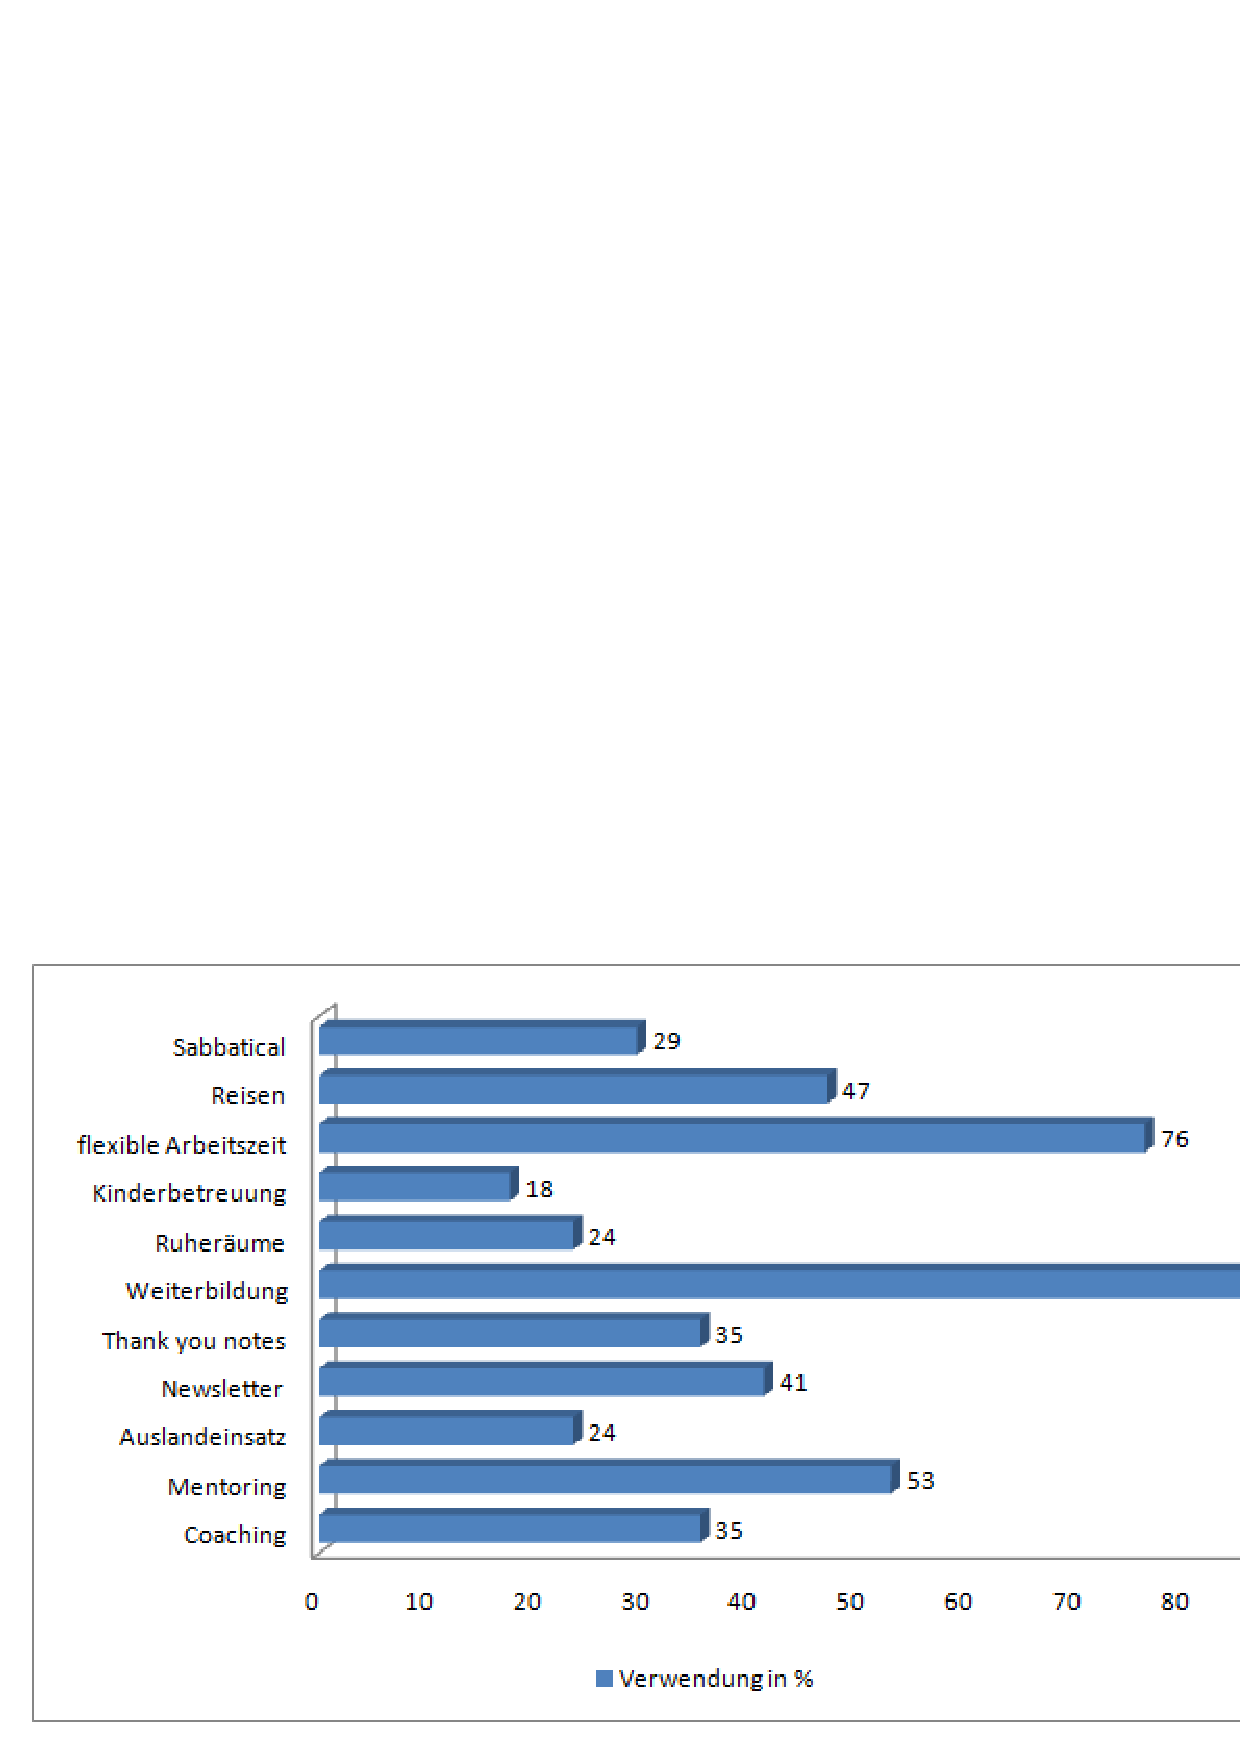
\includegraphics[width=0.9\textwidth]{chap12-unternehmen-anreizverwendung.png}
	\else	
		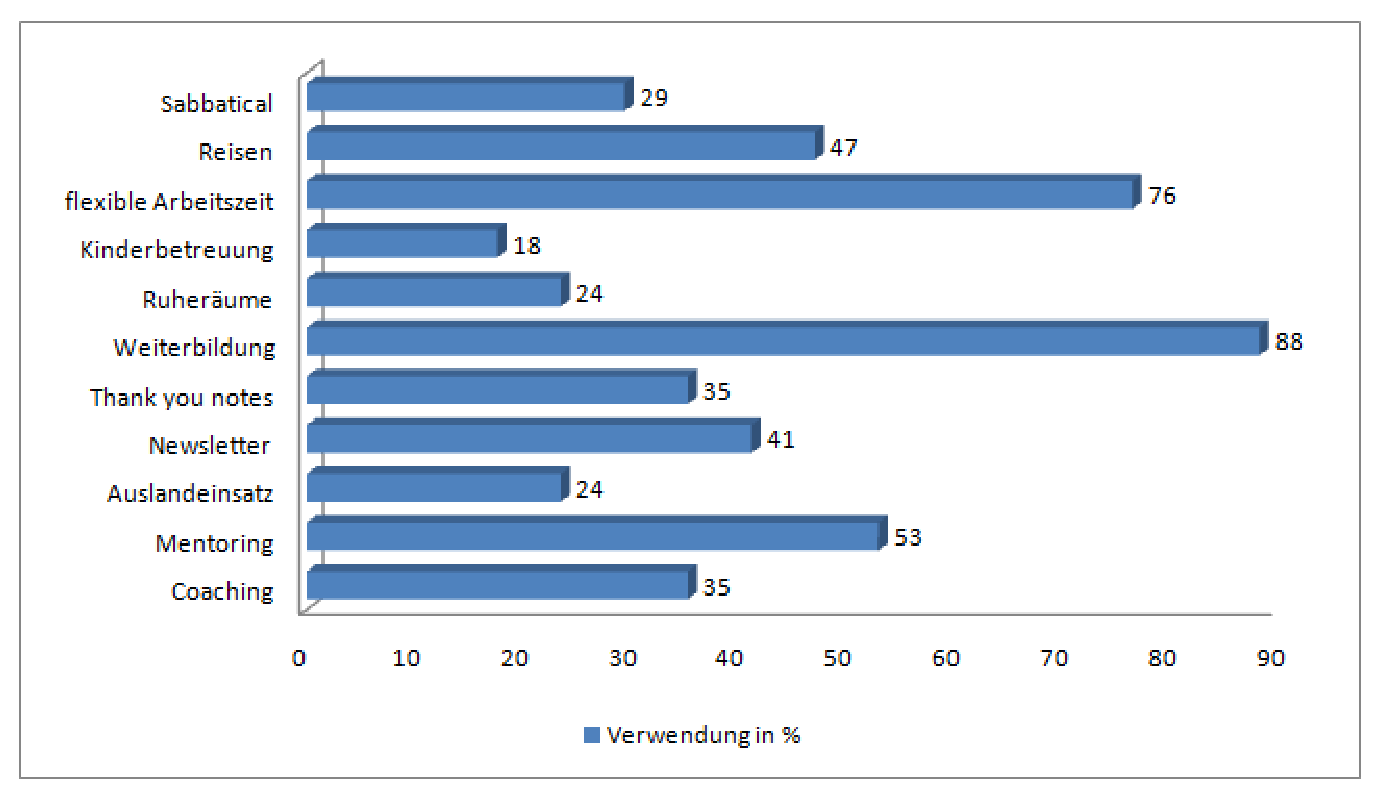
\includegraphics[width=0.9\textwidth]{chap12-unternehmen-anreizverwendung.eps}
	\fi
		
	\caption[Prozentualer Einsatz von Anreizen]{Prozentualer Einsatz von Anreizen (eigene Darstellung)}	
	\label{fig:usageInPercentage}
\end{figure}

\begin{figure}[h]
	\centering
		
	\ifpdf
		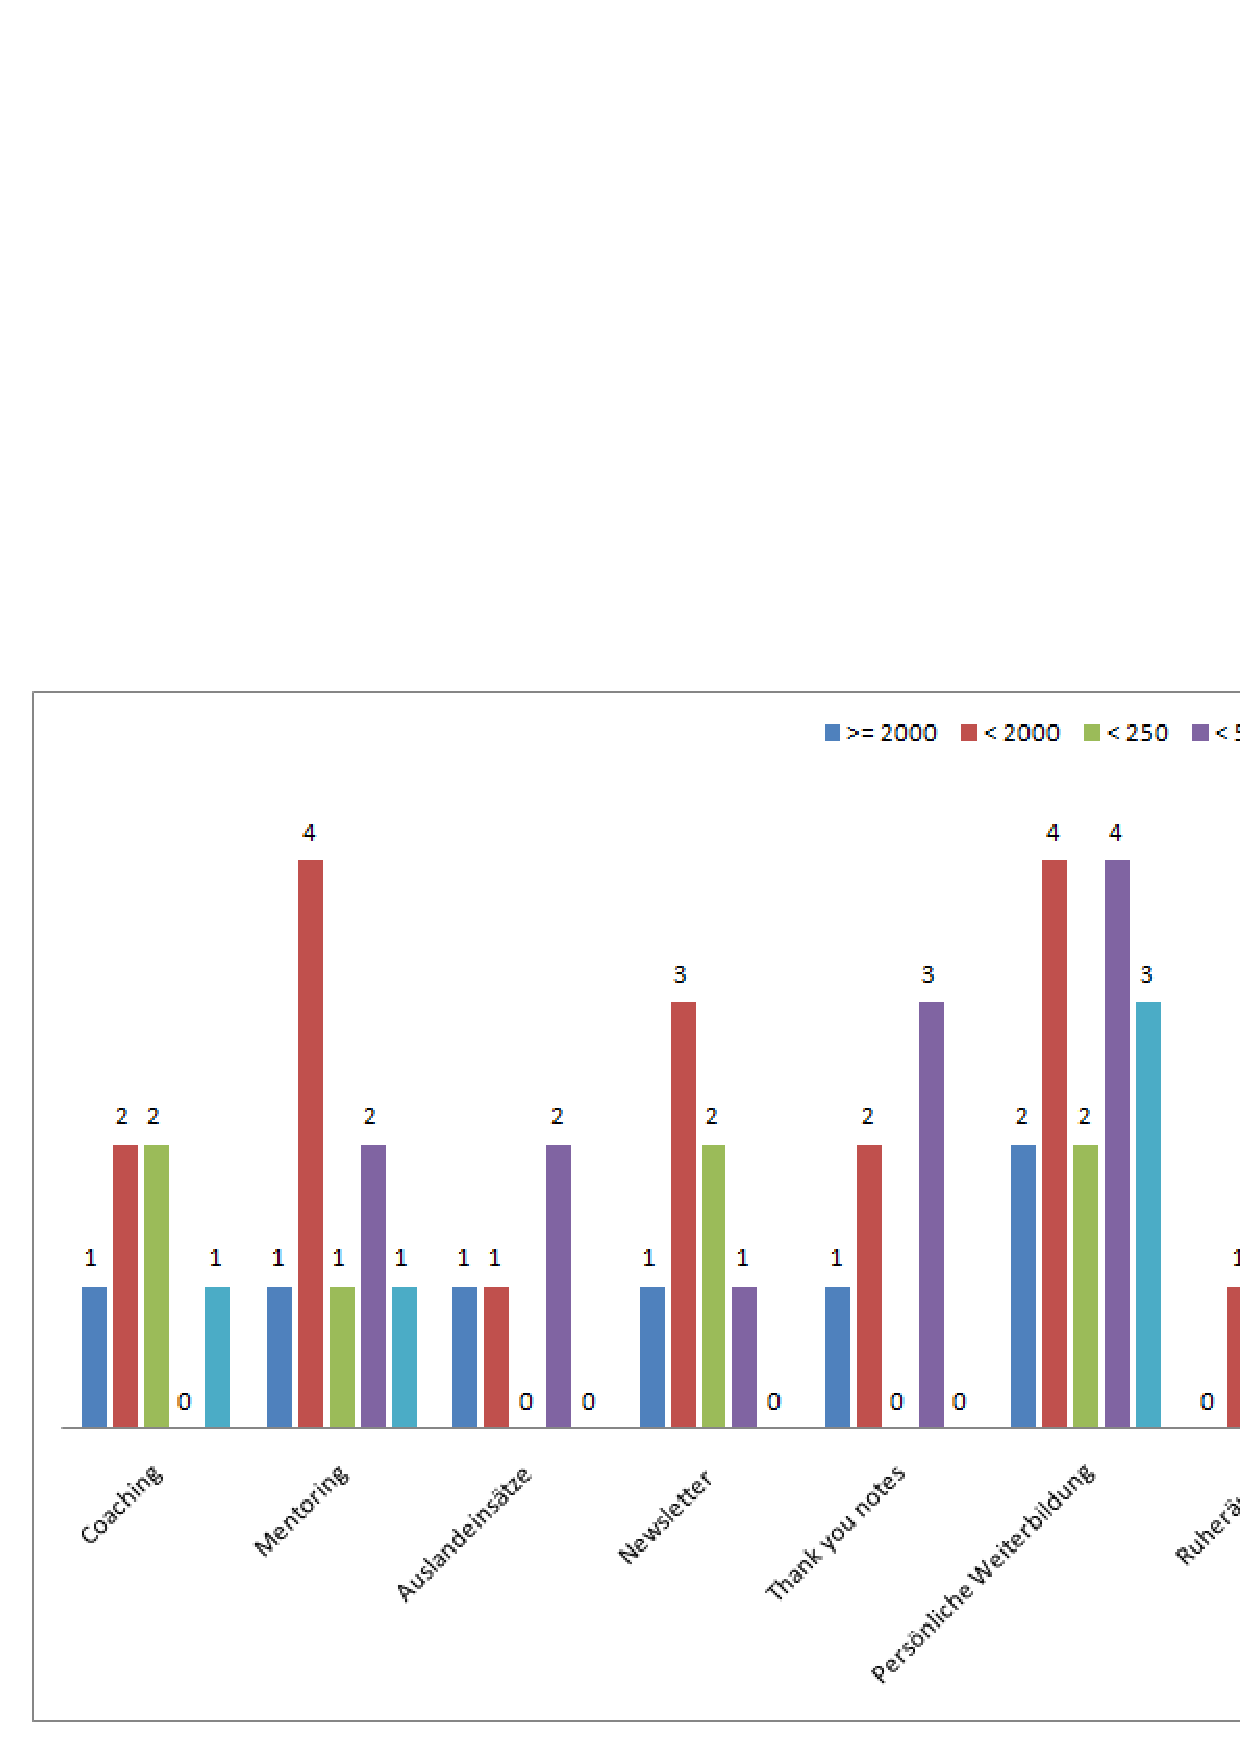
\includegraphics[width=0.9\textwidth]{chap12-unternehmen-anreiz-firmengroesse.png}
	\else	
		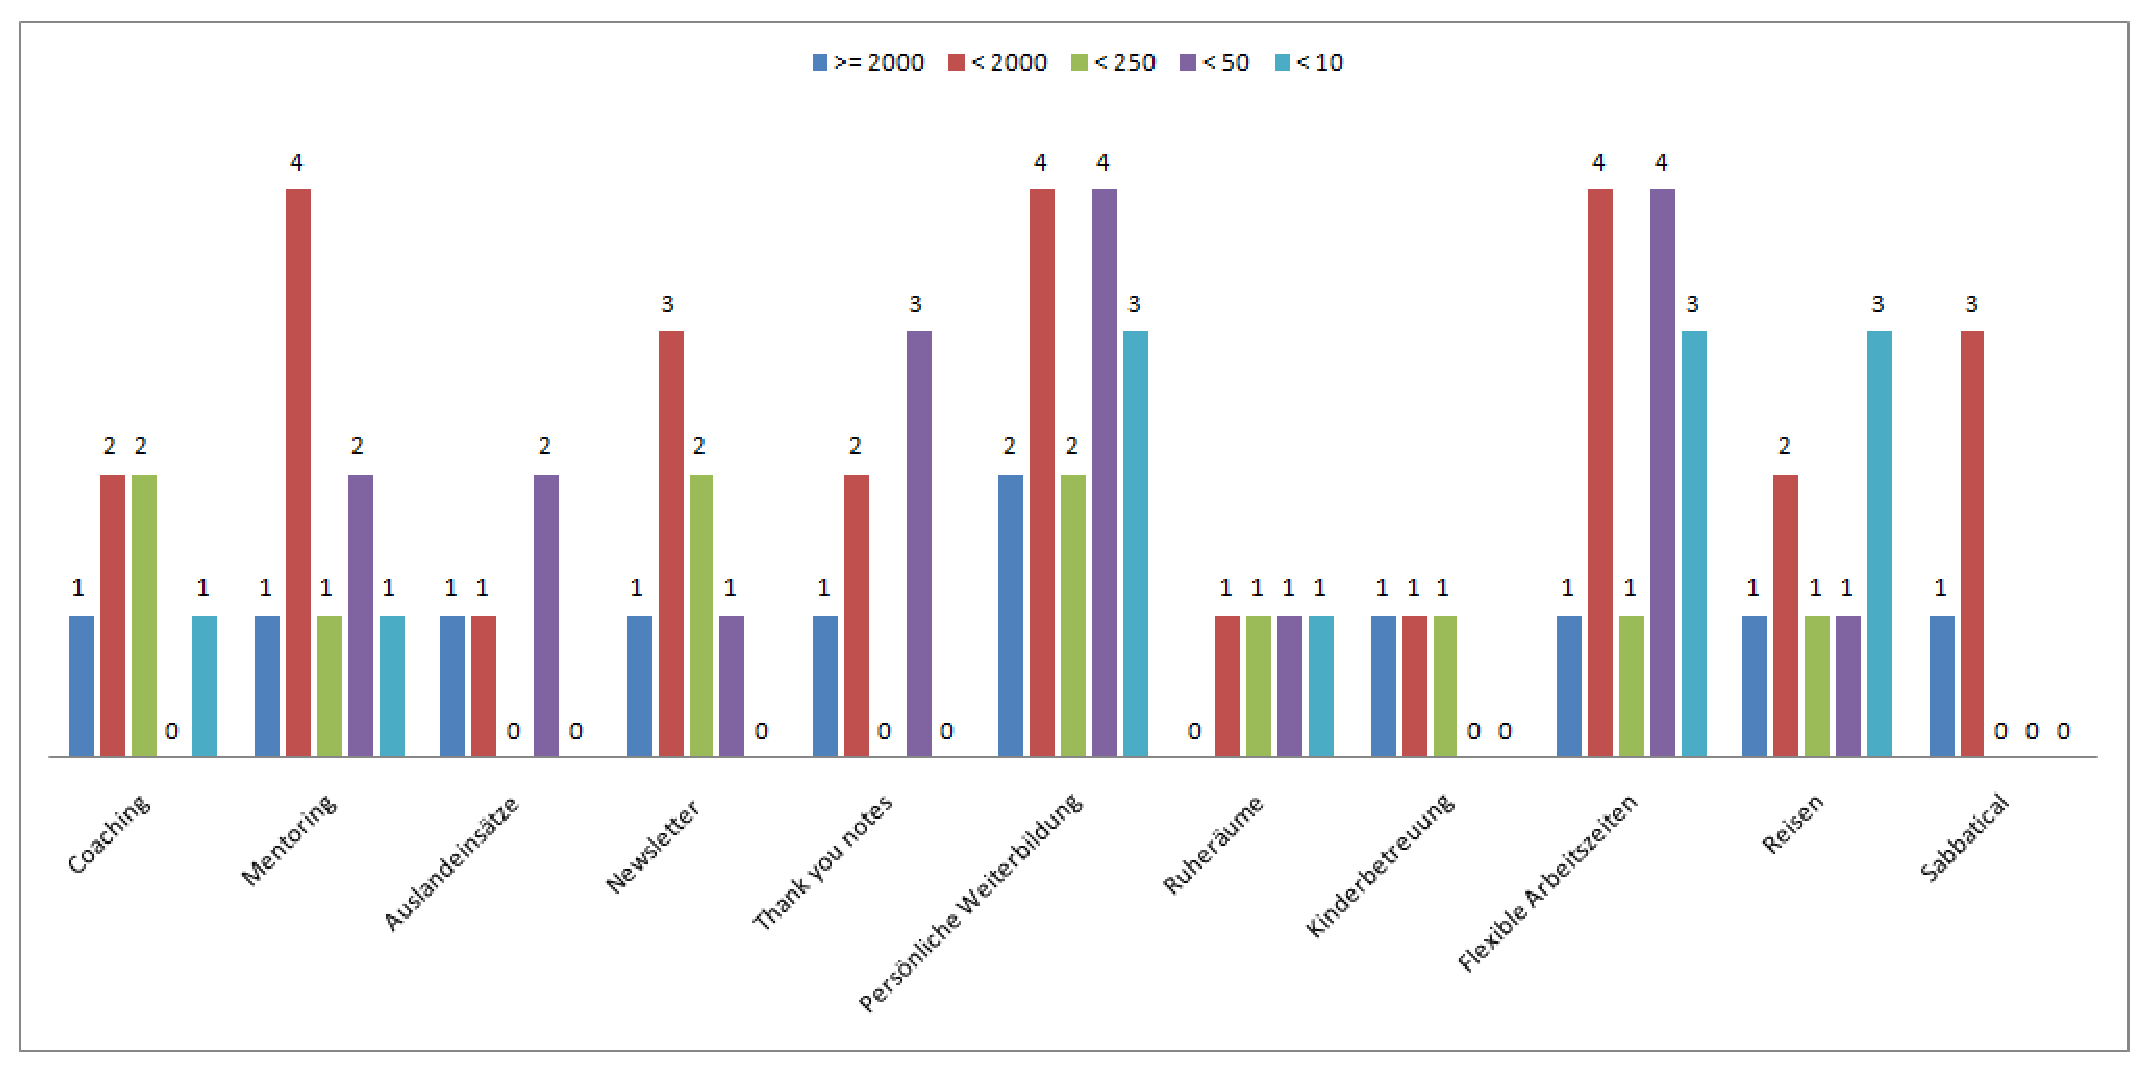
\includegraphics[width=0.9\textwidth]{chap12-unternehmen-anreiz-firmengroesse.eps}
	\fi
		
	\caption[Verwendete Anreize je Unternehmensgr�sse]{Verwendete Anreize je Unternehmensgr�sse (eigene Darstellung)}	
	\label{fig:overallUsageByCompanySize}
\end{figure}

\begin{figure}[h]
	\centering
		
	\ifpdf
		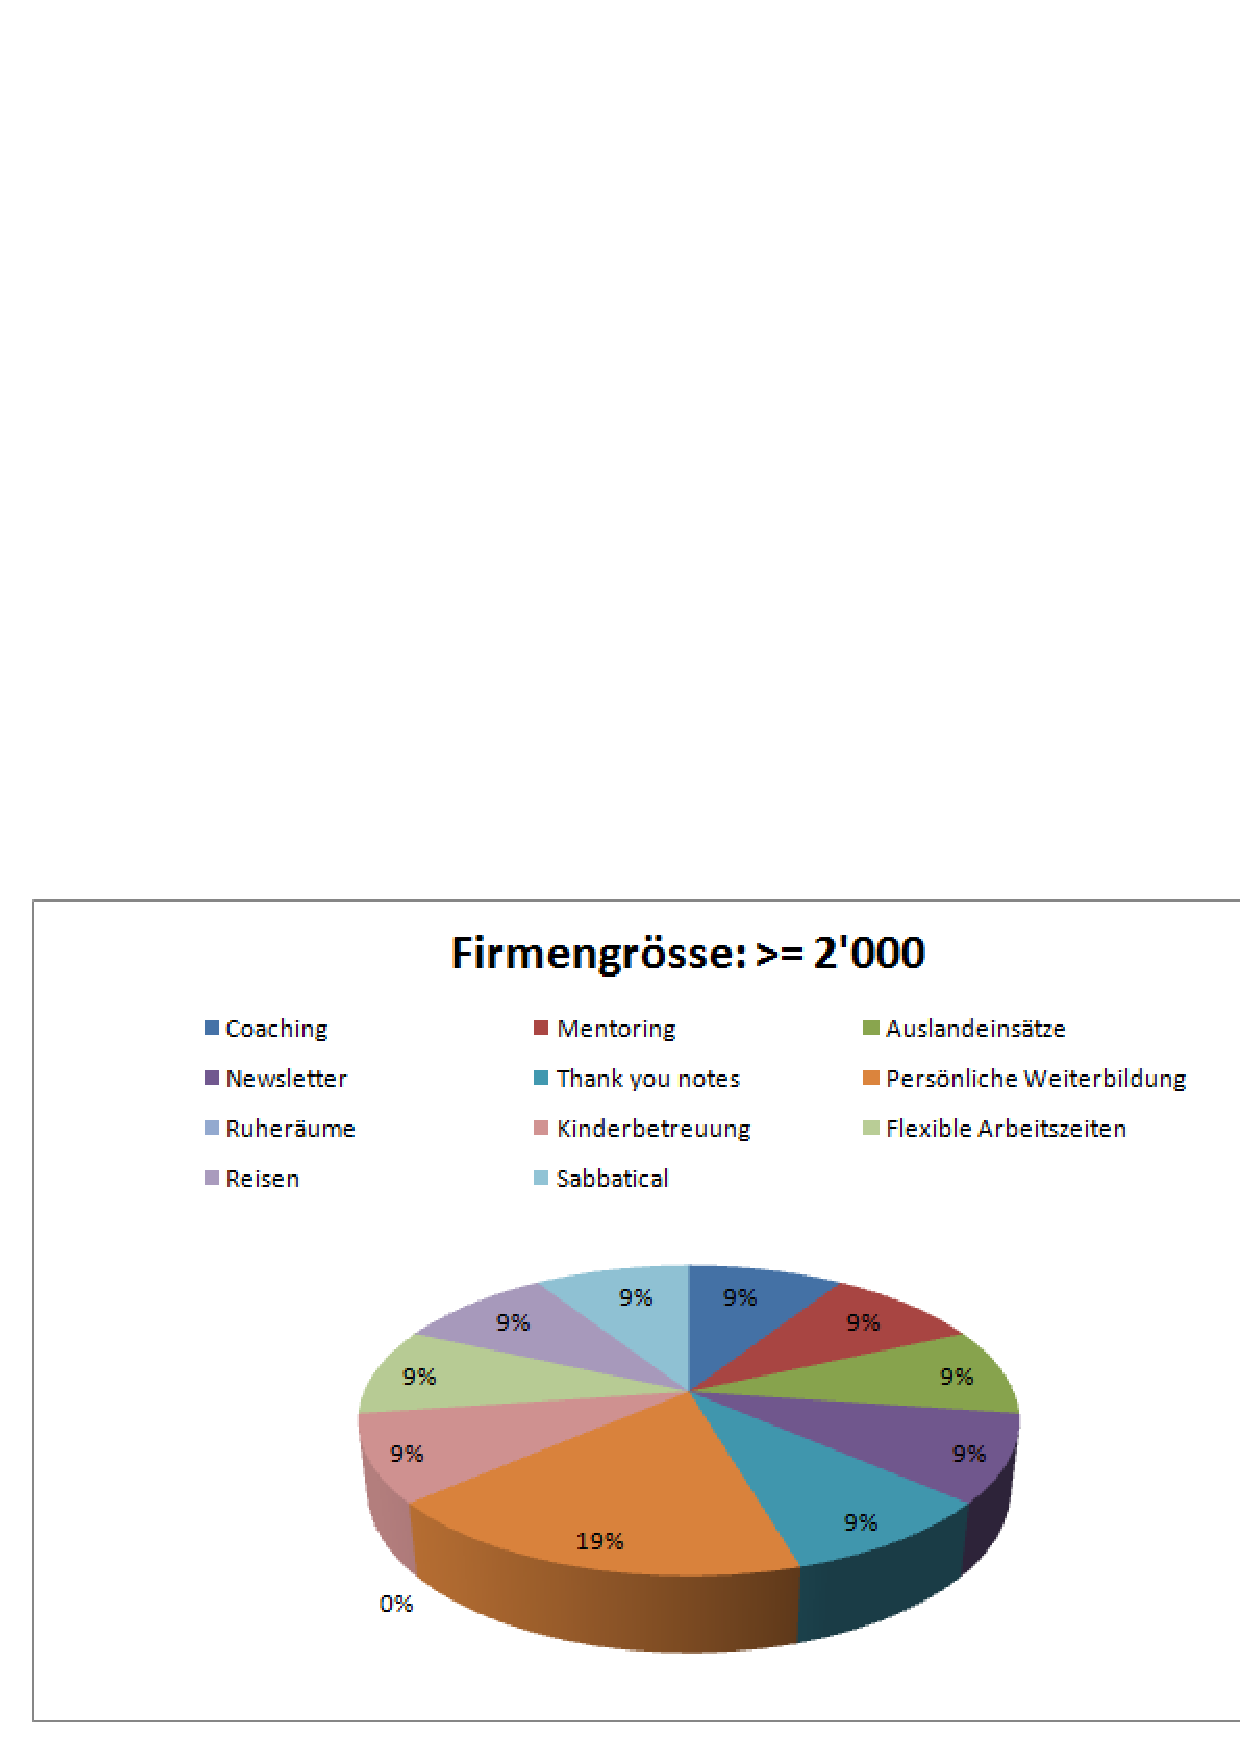
\includegraphics[width=0.9\textwidth]{chap12-unternehmen-usageSizeGt2000.png}
	\else	
		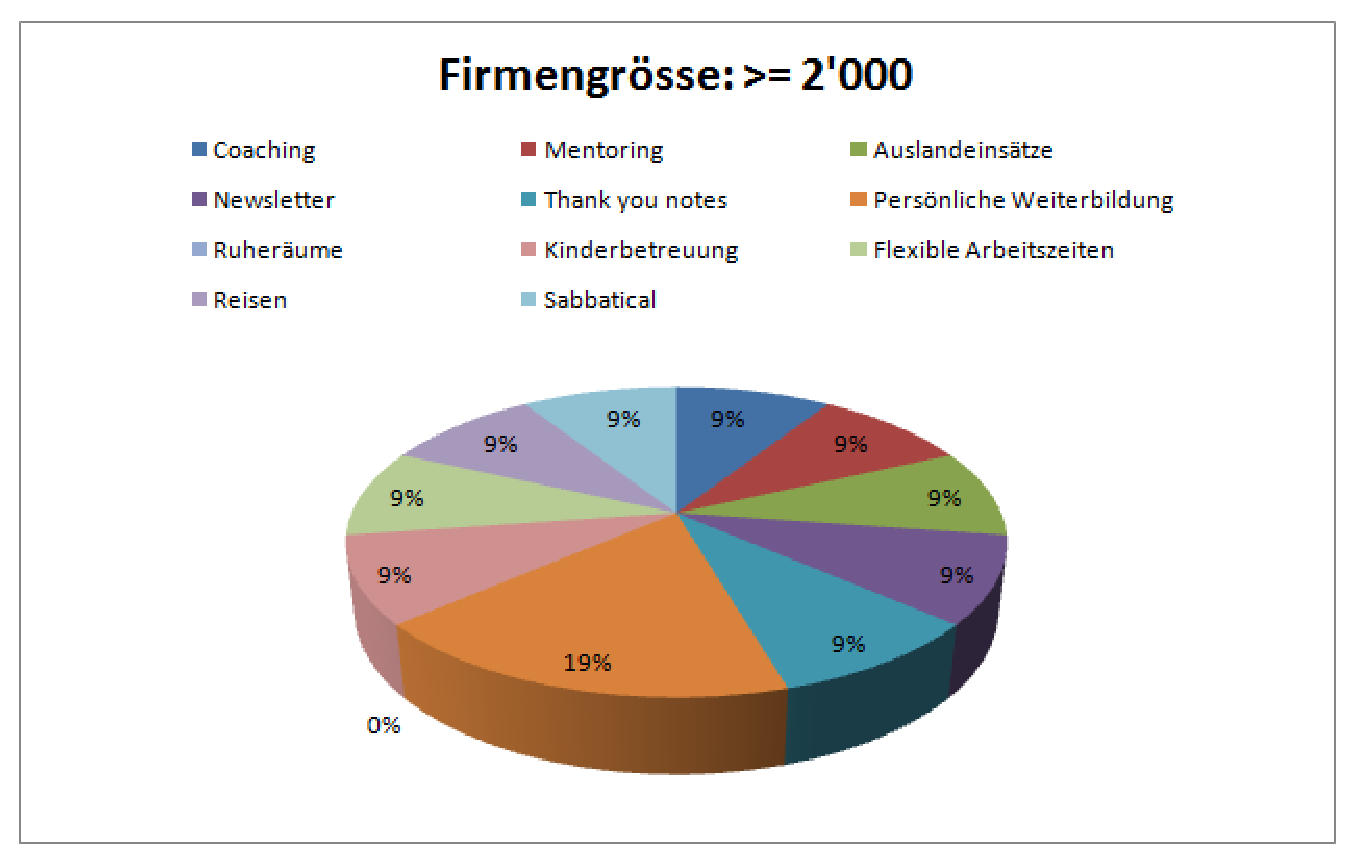
\includegraphics[width=0.9\textwidth]{chap12-unternehmen-usageSizeGt2000.eps}
	\fi
		
	\caption[Verwendete Anreize bei mehr als 2'000 Mitarbeiter]{Verwendete Anreize bei mehr als 2'000 Mitarbeiter (eigene Darstellung)}	
	\label{fig:overallUsageByCompanySizeGt2000}
\end{figure}

\begin{figure}[h]
	\centering
		
	\ifpdf
		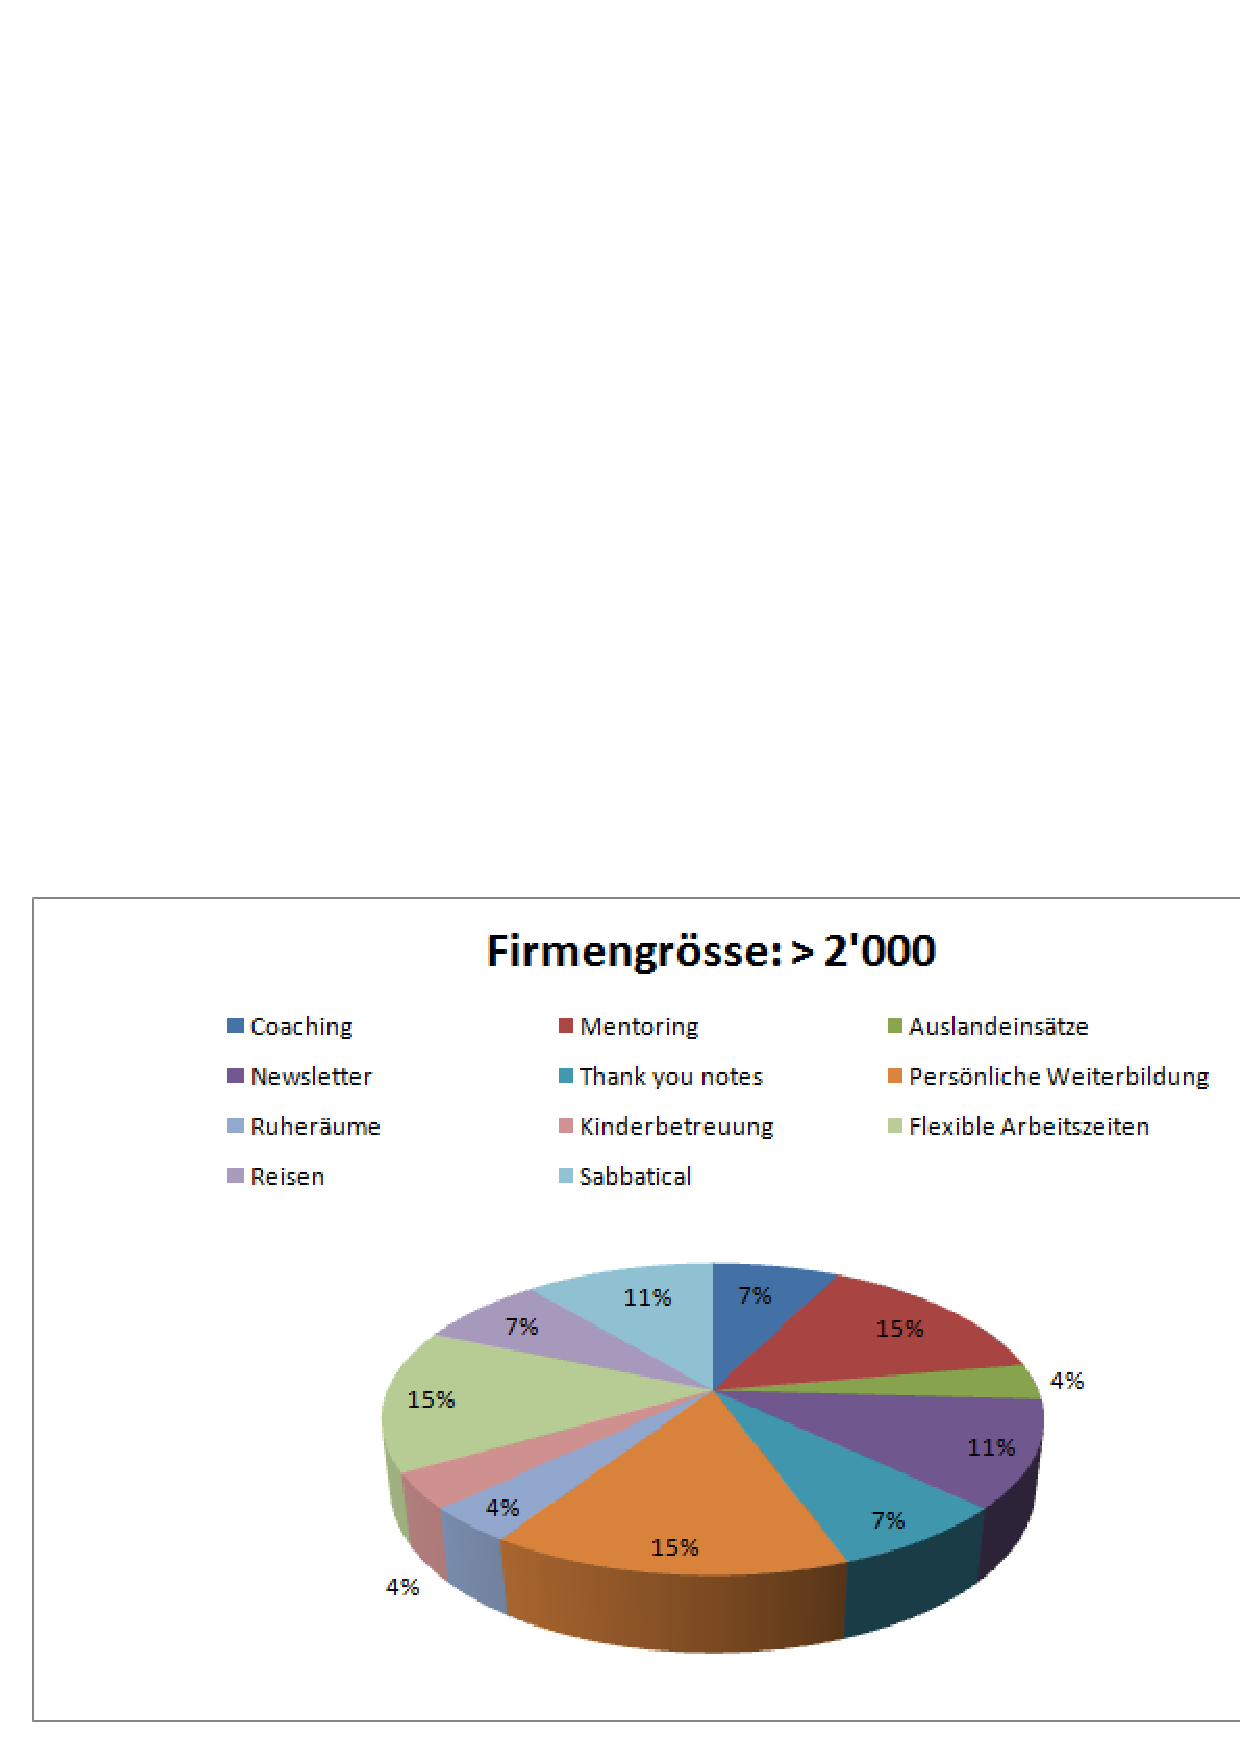
\includegraphics[width=0.9\textwidth]{chap12-unternehmen-usageSizeLt2000.png}
	\else	
		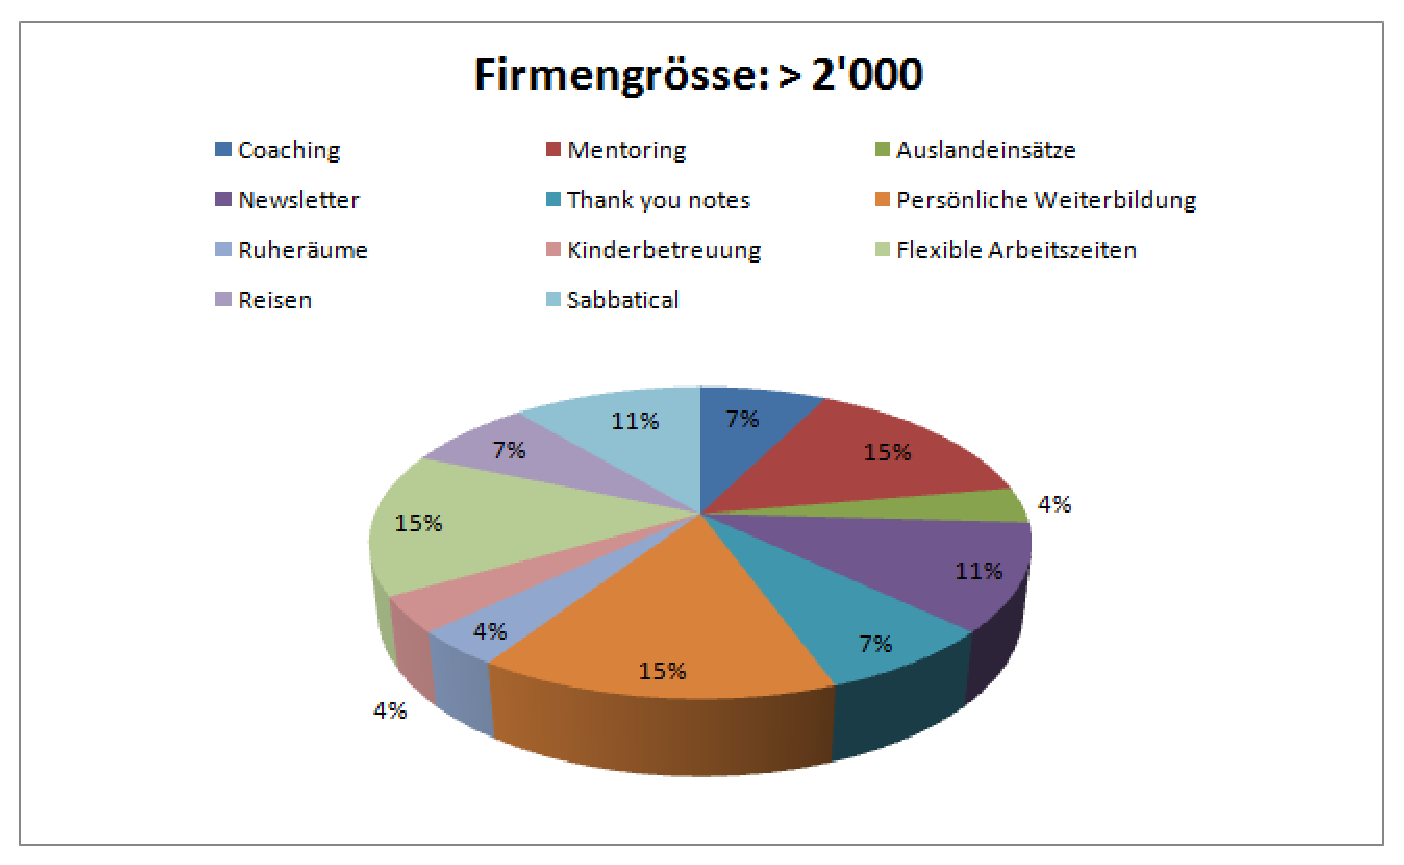
\includegraphics[width=0.9\textwidth]{chap12-unternehmen-usageSizeLt2000.eps}
	\fi
		
	\caption[Verwendete Anreize bei bis zu 2'000 Mitarbeiter]{Verwendete Anreize bei bis zu 2'000 Mitarbeiter (eigene Darstellung)}	
	\label{fig:overallUsageByCompanySizeLt2000}
\end{figure}

\begin{figure}[h]
	\centering
		
	\ifpdf
		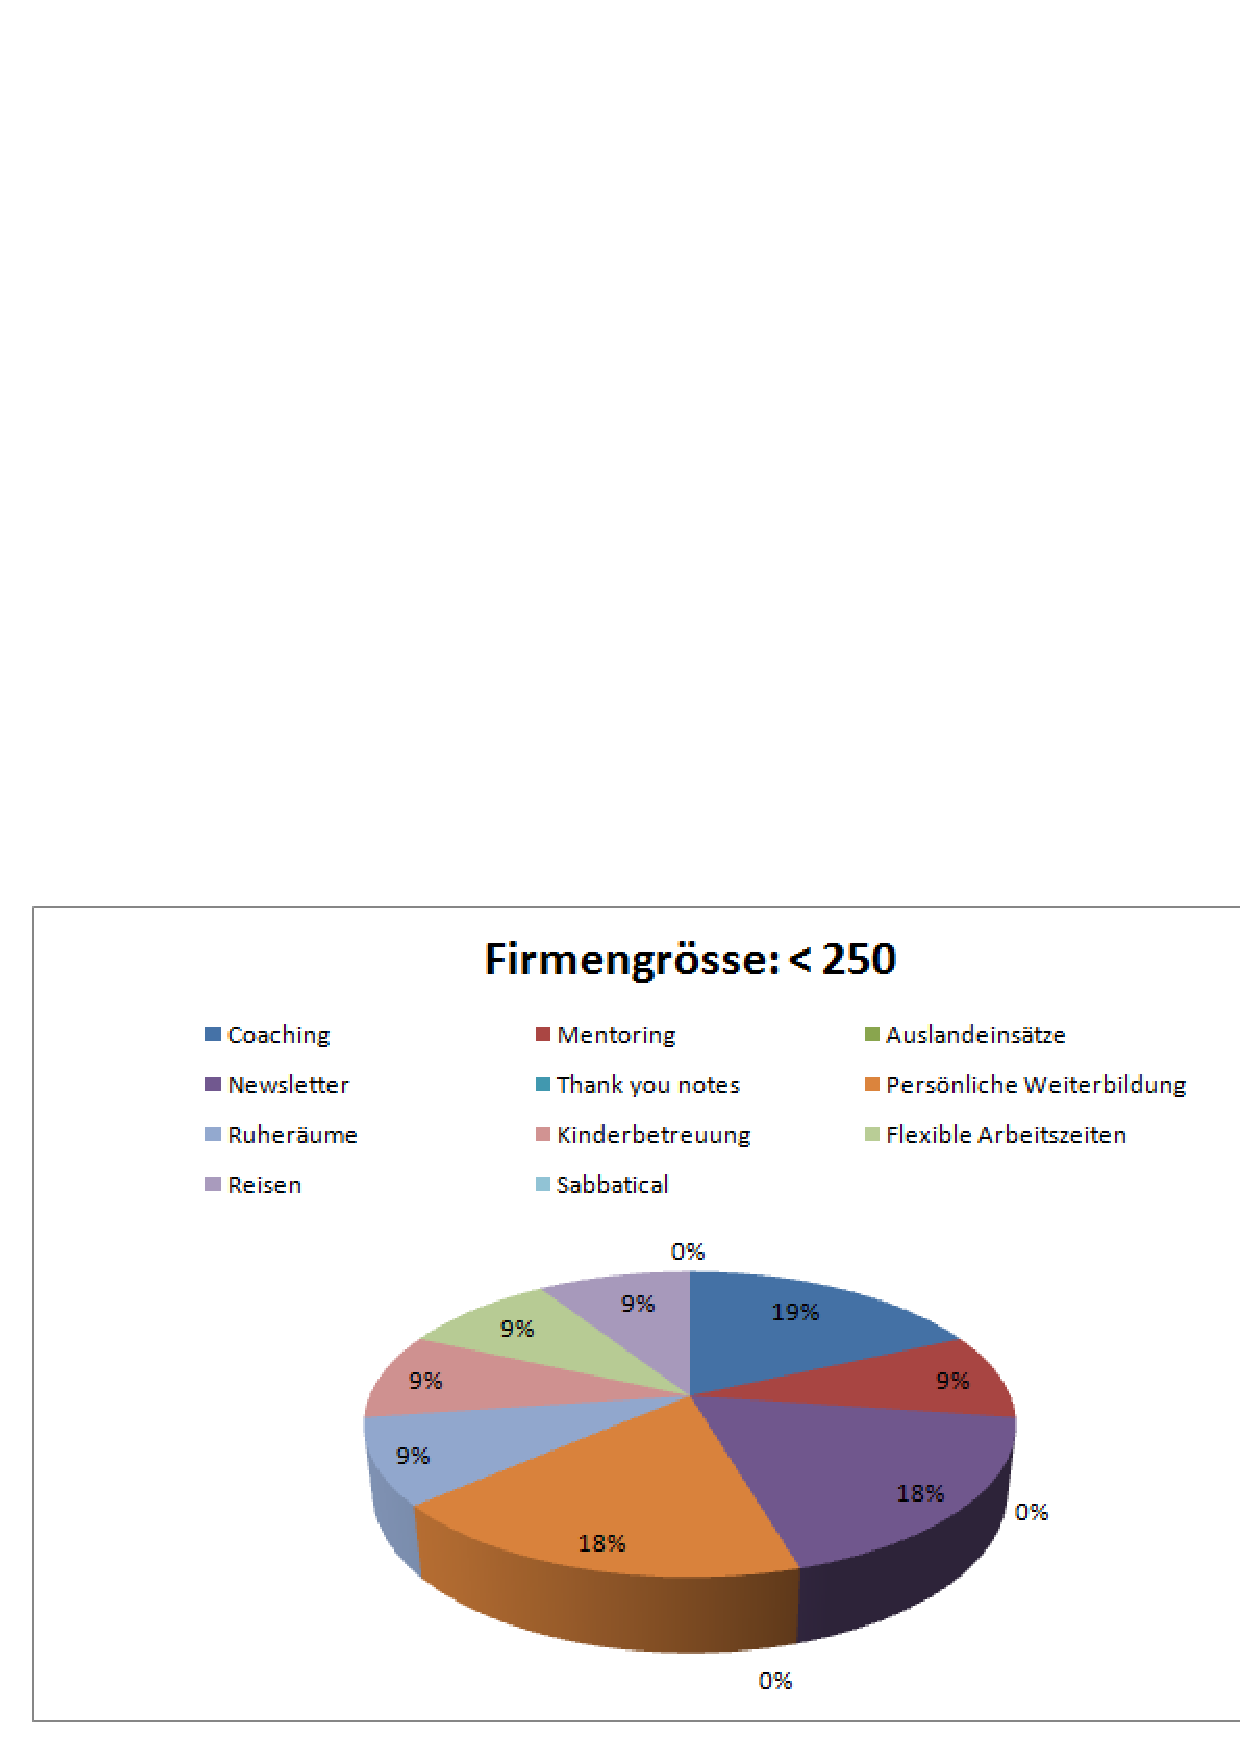
\includegraphics[width=0.9\textwidth]{chap12-unternehmen-usageSizeLt250.png}
	\else	
		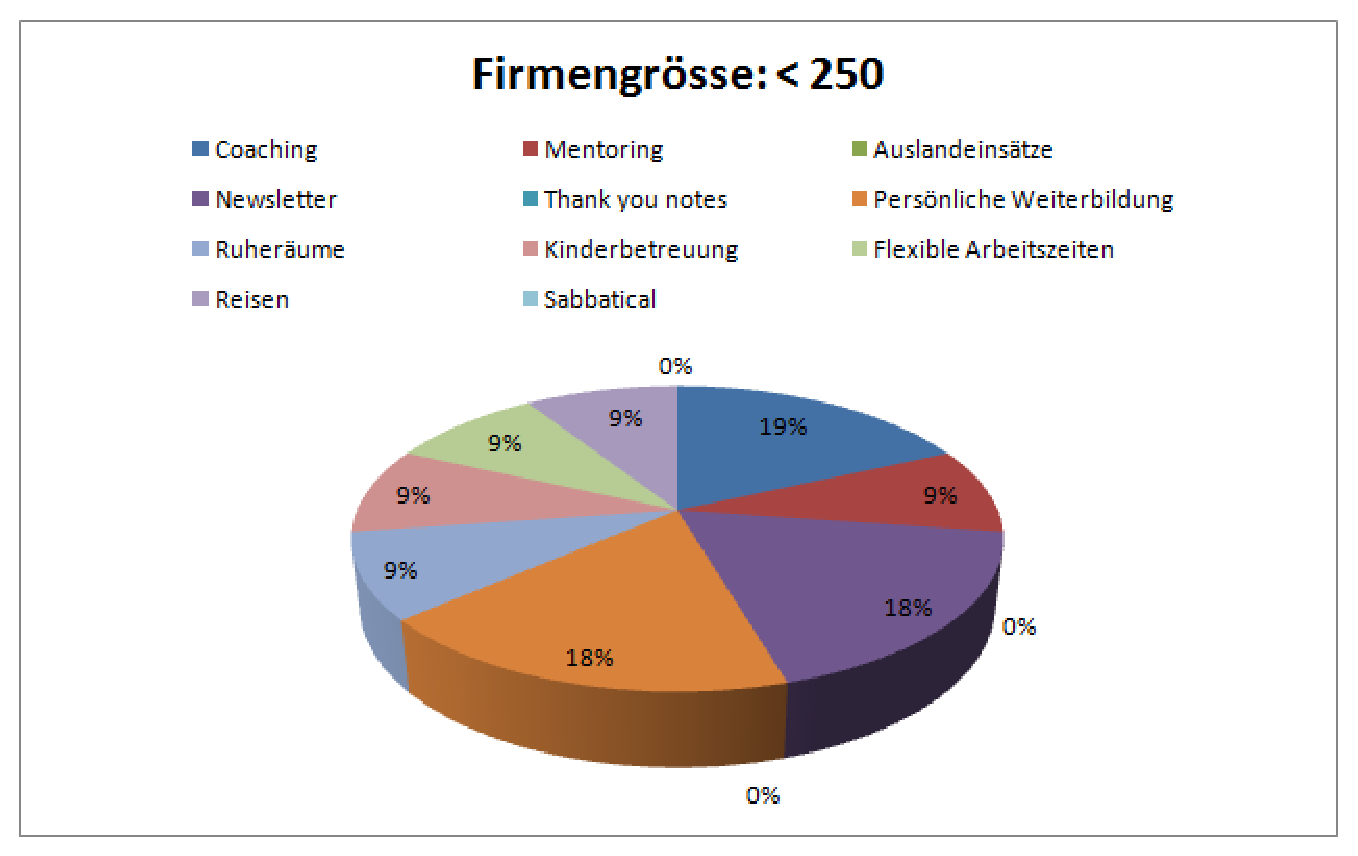
\includegraphics[width=0.9\textwidth]{chap12-unternehmen-usageSizeLt250.eps}
	\fi
		
	\caption[Verwendete Anreize bei bis zu 250 Mitarbeiter]{Verwendete Anreize bei bis zu 250 Mitarbeiter (eigene Darstellung)}	
	\label{fig:overallUsageByCompanySizeLt250}
\end{figure}

\begin{figure}[h]
	\centering
		
	\ifpdf
		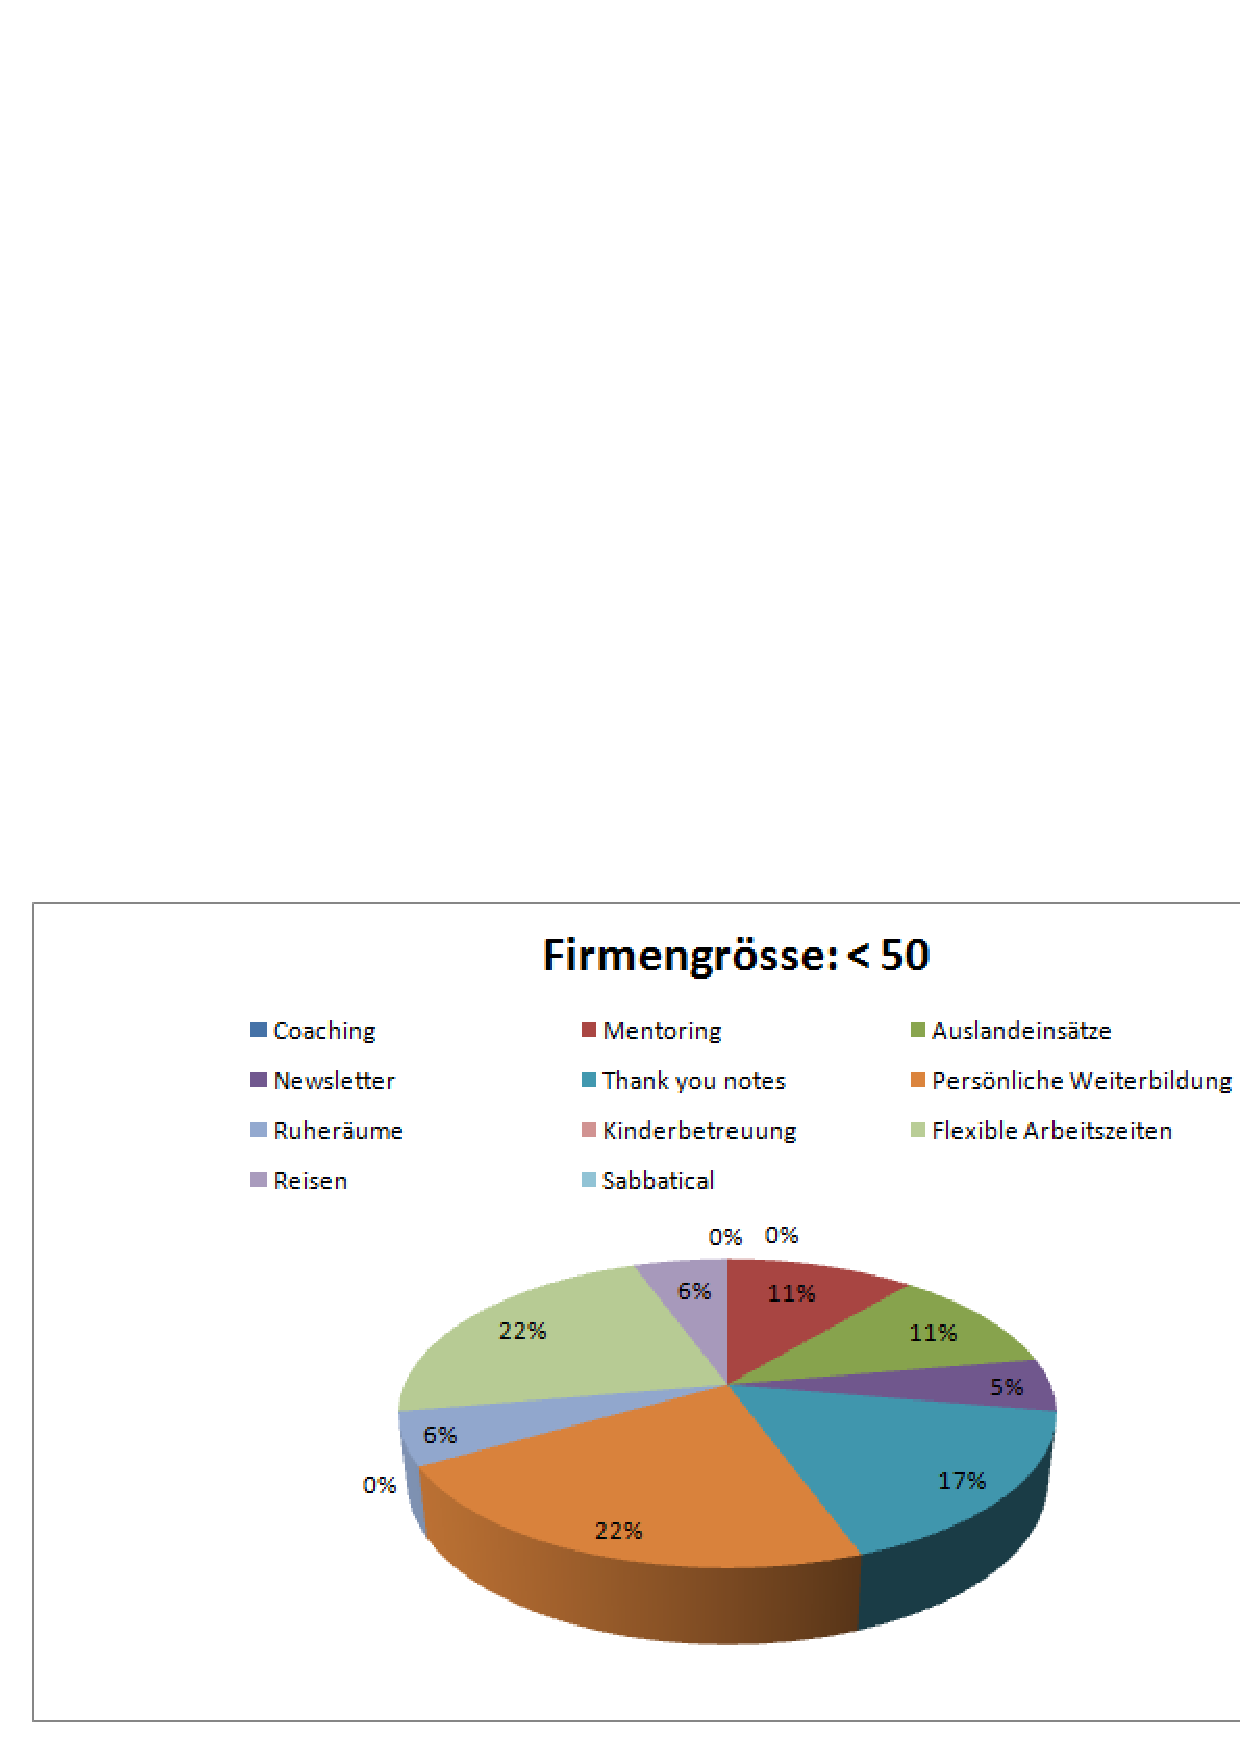
\includegraphics[width=0.9\textwidth]{chap12-unternehmen-usageSizeLt50.png}
	\else	
		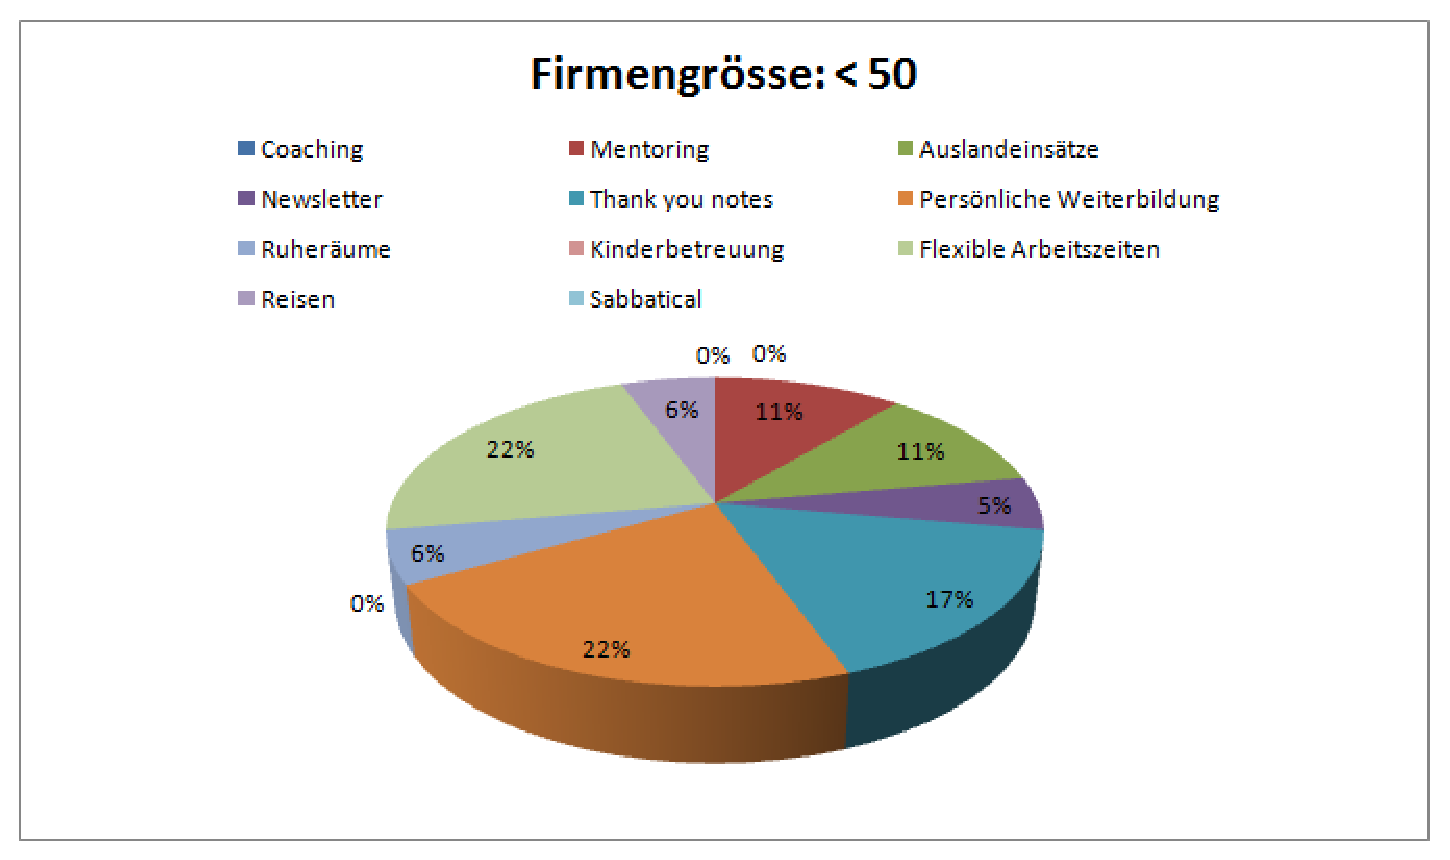
\includegraphics[width=0.9\textwidth]{chap12-unternehmen-usageSizeLt50.eps}
	\fi
		
	\caption[Verwendete Anreize bei bis zu 50 Mitarbeiter]{Verwendete Anreize bei bis zu 50 Mitarbeiter (eigene Darstellung)}	
	\label{fig:overallUsageByCompanySizeLt50}
\end{figure}

\begin{figure}[h]
	\centering
		
	\ifpdf
		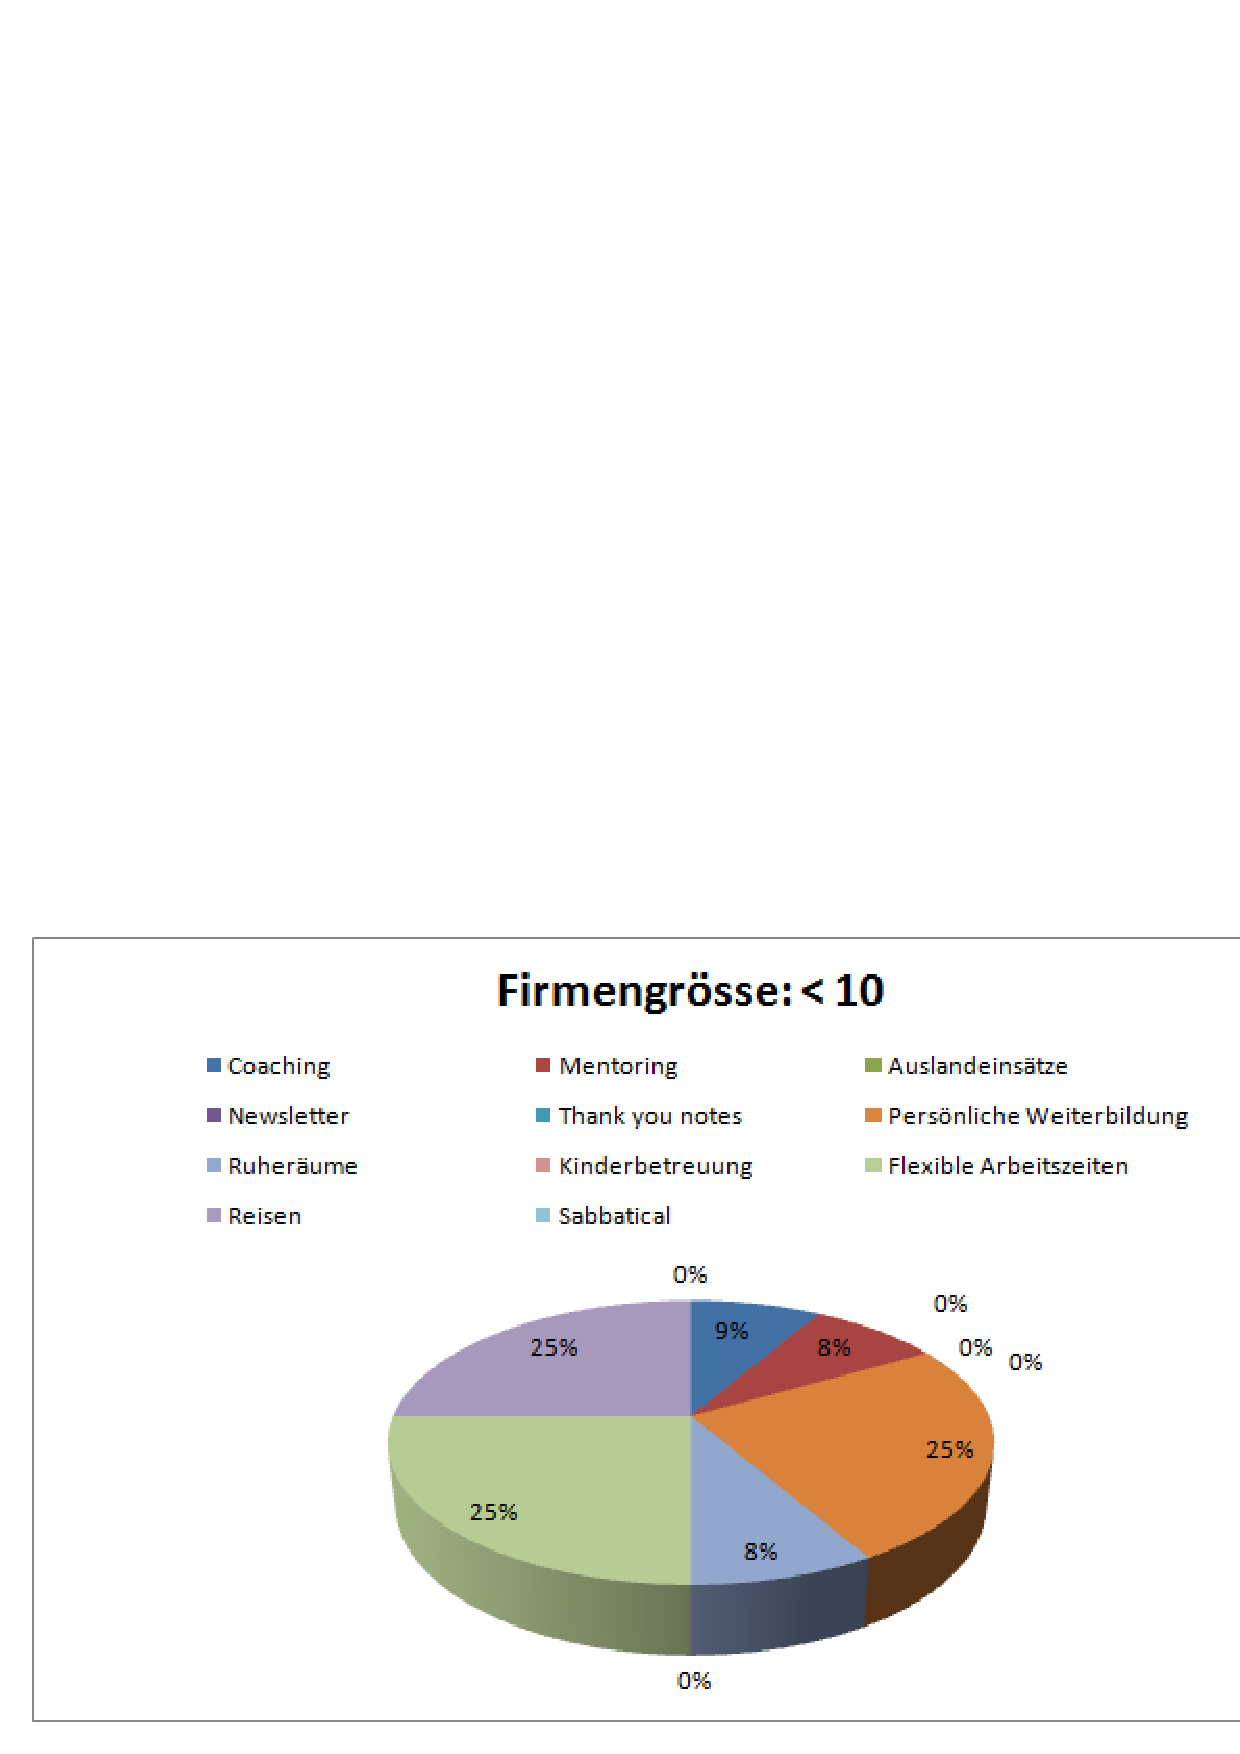
\includegraphics[width=0.9\textwidth]{chap12-unternehmen-usageSizeLt10.png}
	\else	
		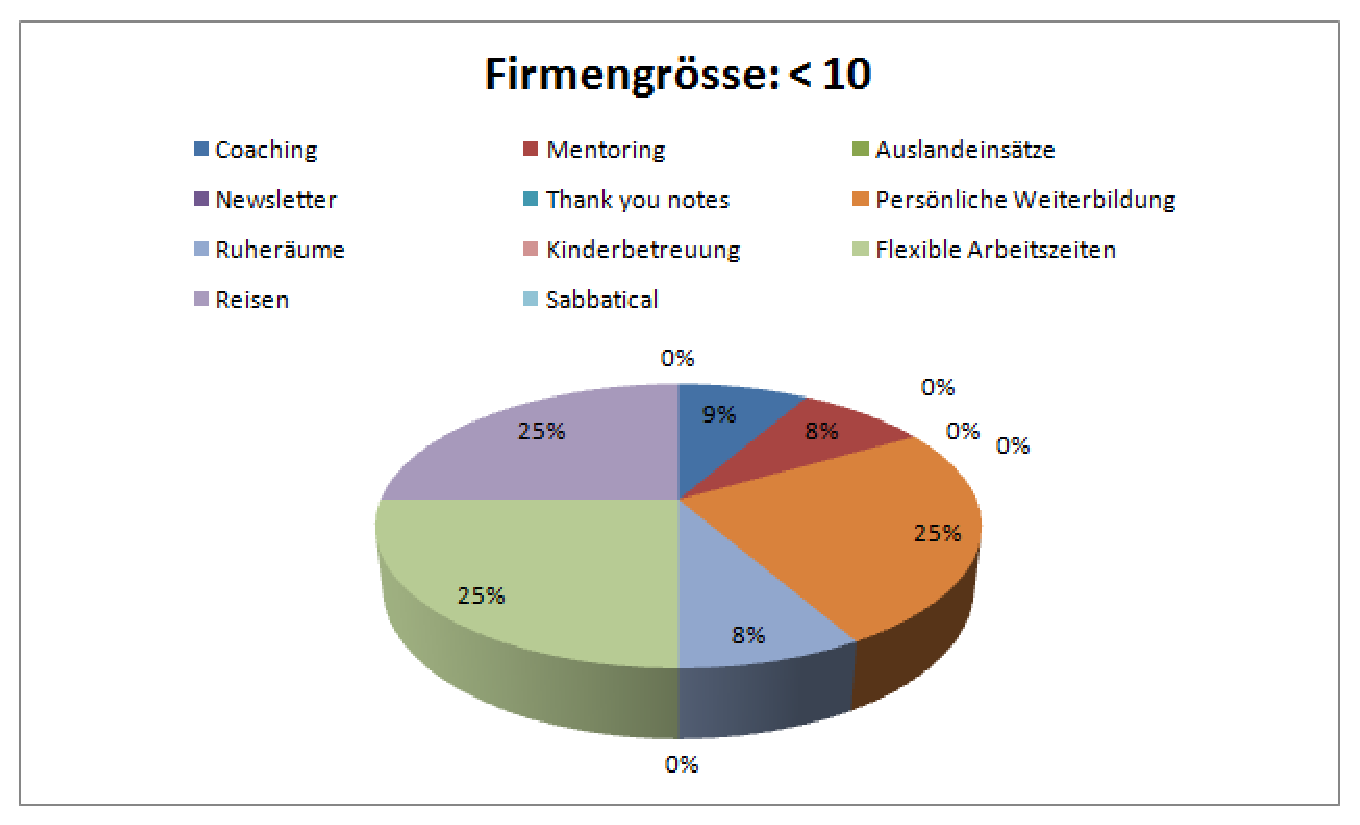
\includegraphics[width=0.9\textwidth]{chap12-unternehmen-usageSizeLt10.eps}
	\fi
		
	\caption[Verwendete Anreize bei bis zu 10 Mitarbeiter]{Verwendete Anreize bei bis zu 10 Mitarbeiter (eigene Darstellung)}	
	\label{fig:overallUsageByCompanySizeLt10}
\end{figure}

\begin{figure}[h]
	\centering
		
	\ifpdf
		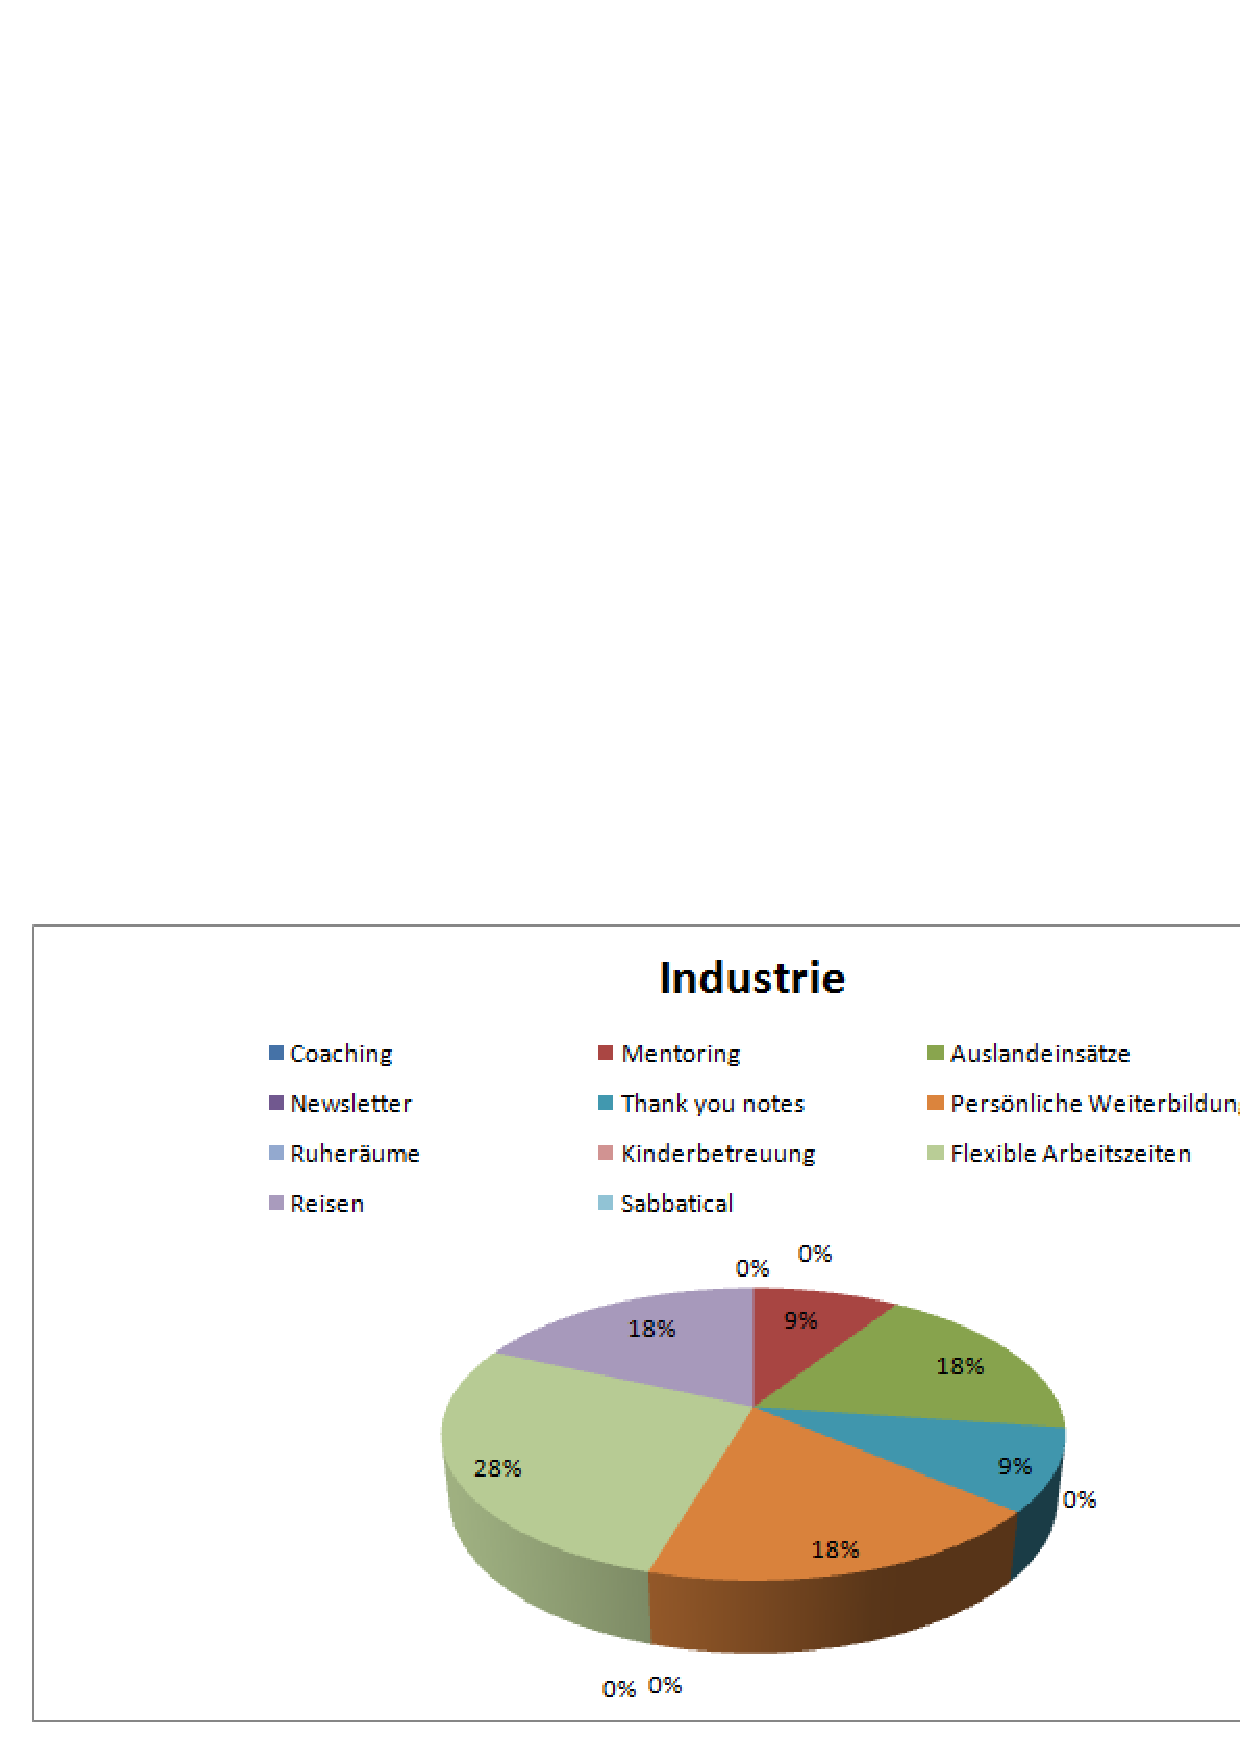
\includegraphics[width=0.9\textwidth]{chap12-unternehmen-anreize-industie.png}
	\else	
		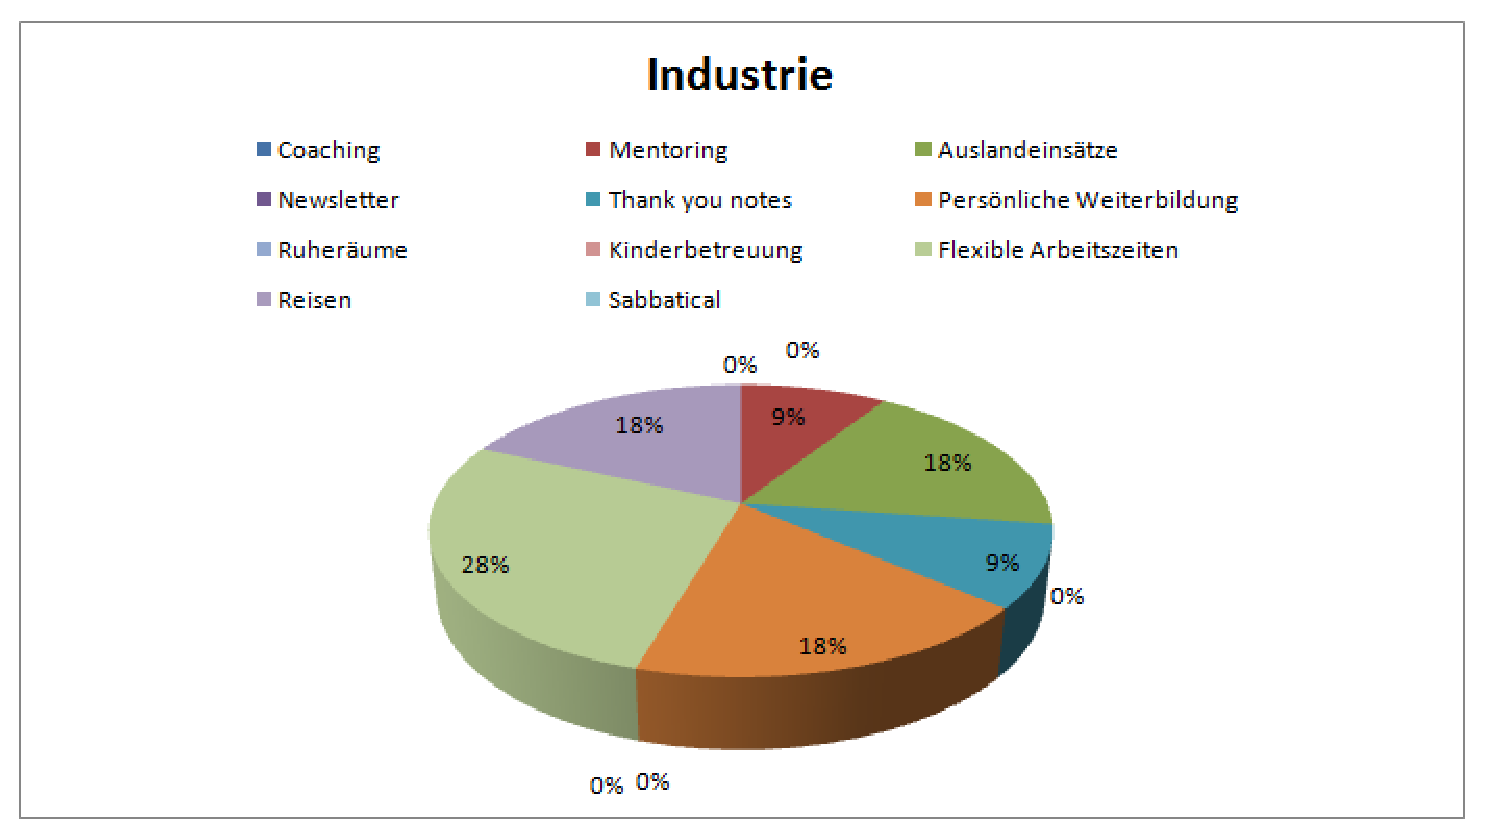
\includegraphics[width=0.9\textwidth]{chap12-unternehmen-anreize-industie.eps}
	\fi
		
	\caption[Verwendete Anreize im Industriesektor]{Verwendete Anreize im Industriesektor (eigene Darstellung)}	
	\label{fig:usageInIndustrySector}
\end{figure}

\begin{figure}[h]
	\centering
		
	\ifpdf
		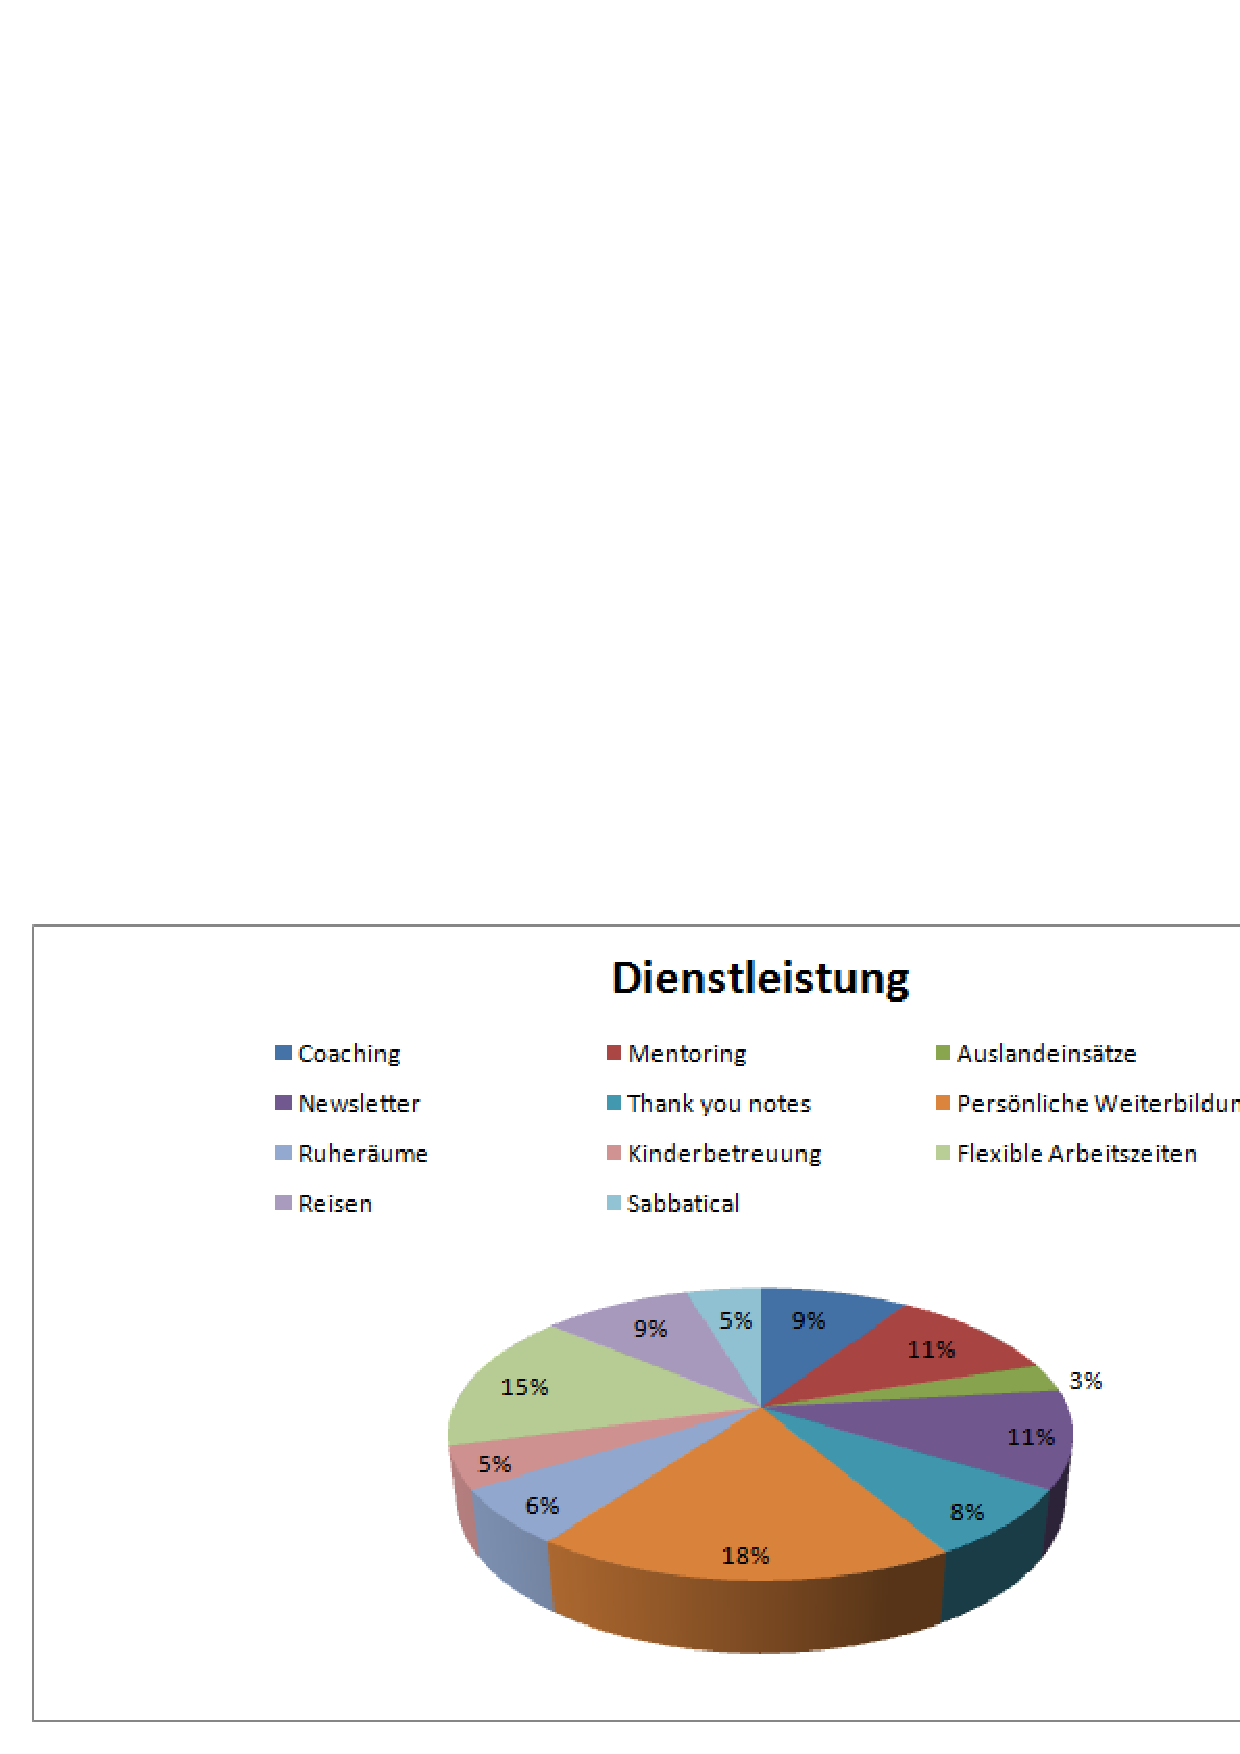
\includegraphics[width=0.9\textwidth]{chap12-unternehmen-anreiz-dienstleistung.png}
	\else	
		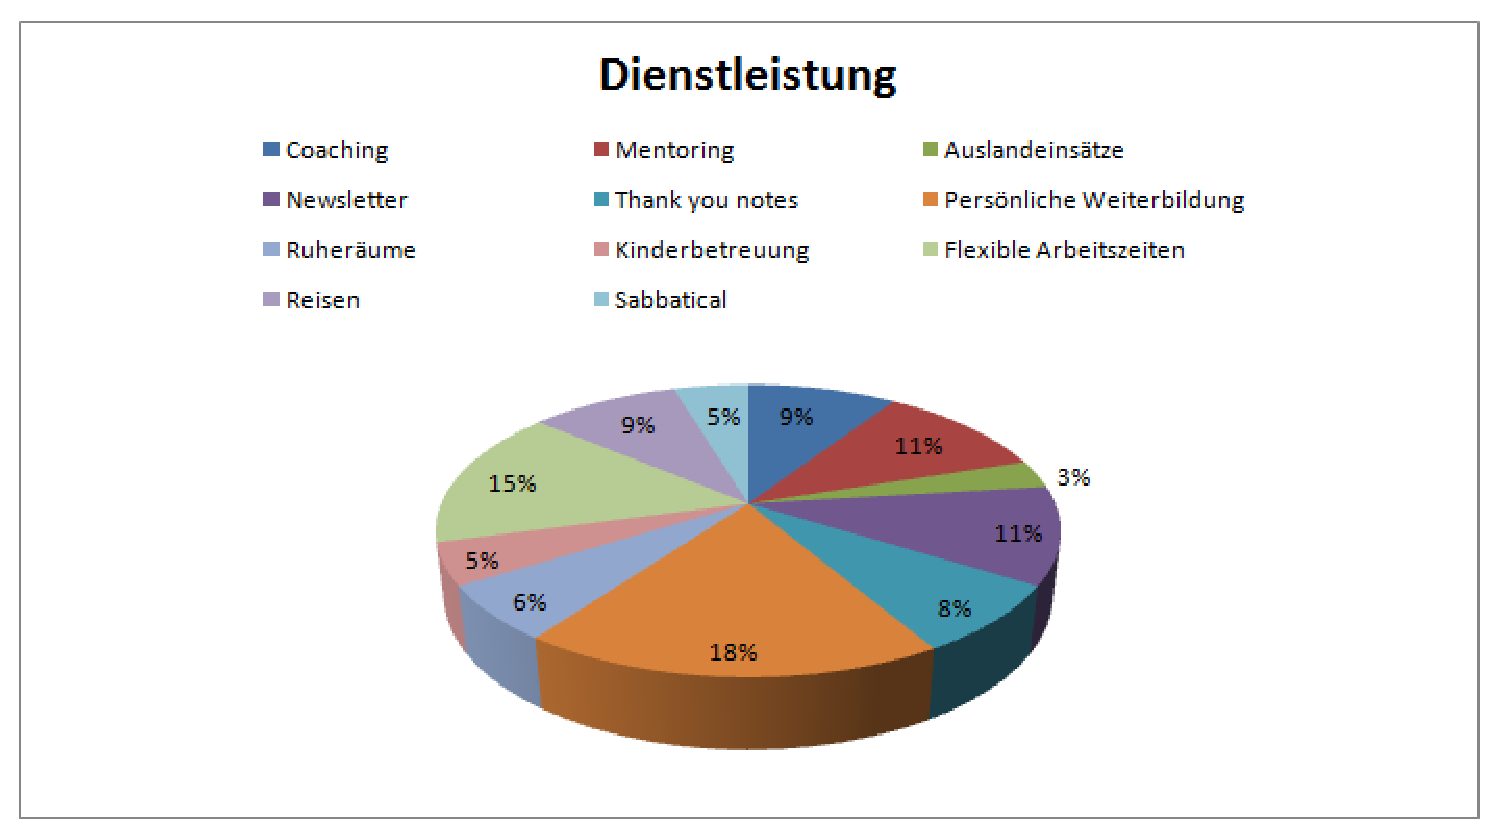
\includegraphics[width=0.9\textwidth]{chap12-unternehmen-anreiz-dienstleistung.eps}
	\fi
		
	\caption[Verwendete Anreize im Industriesektor]{Verwendete Anreize im Industriesektor (eigene Darstellung)}	
	\label{fig:usageInServiceSector}
\end{figure}

\begin{figure}[h]
	\centering
		
	\ifpdf
		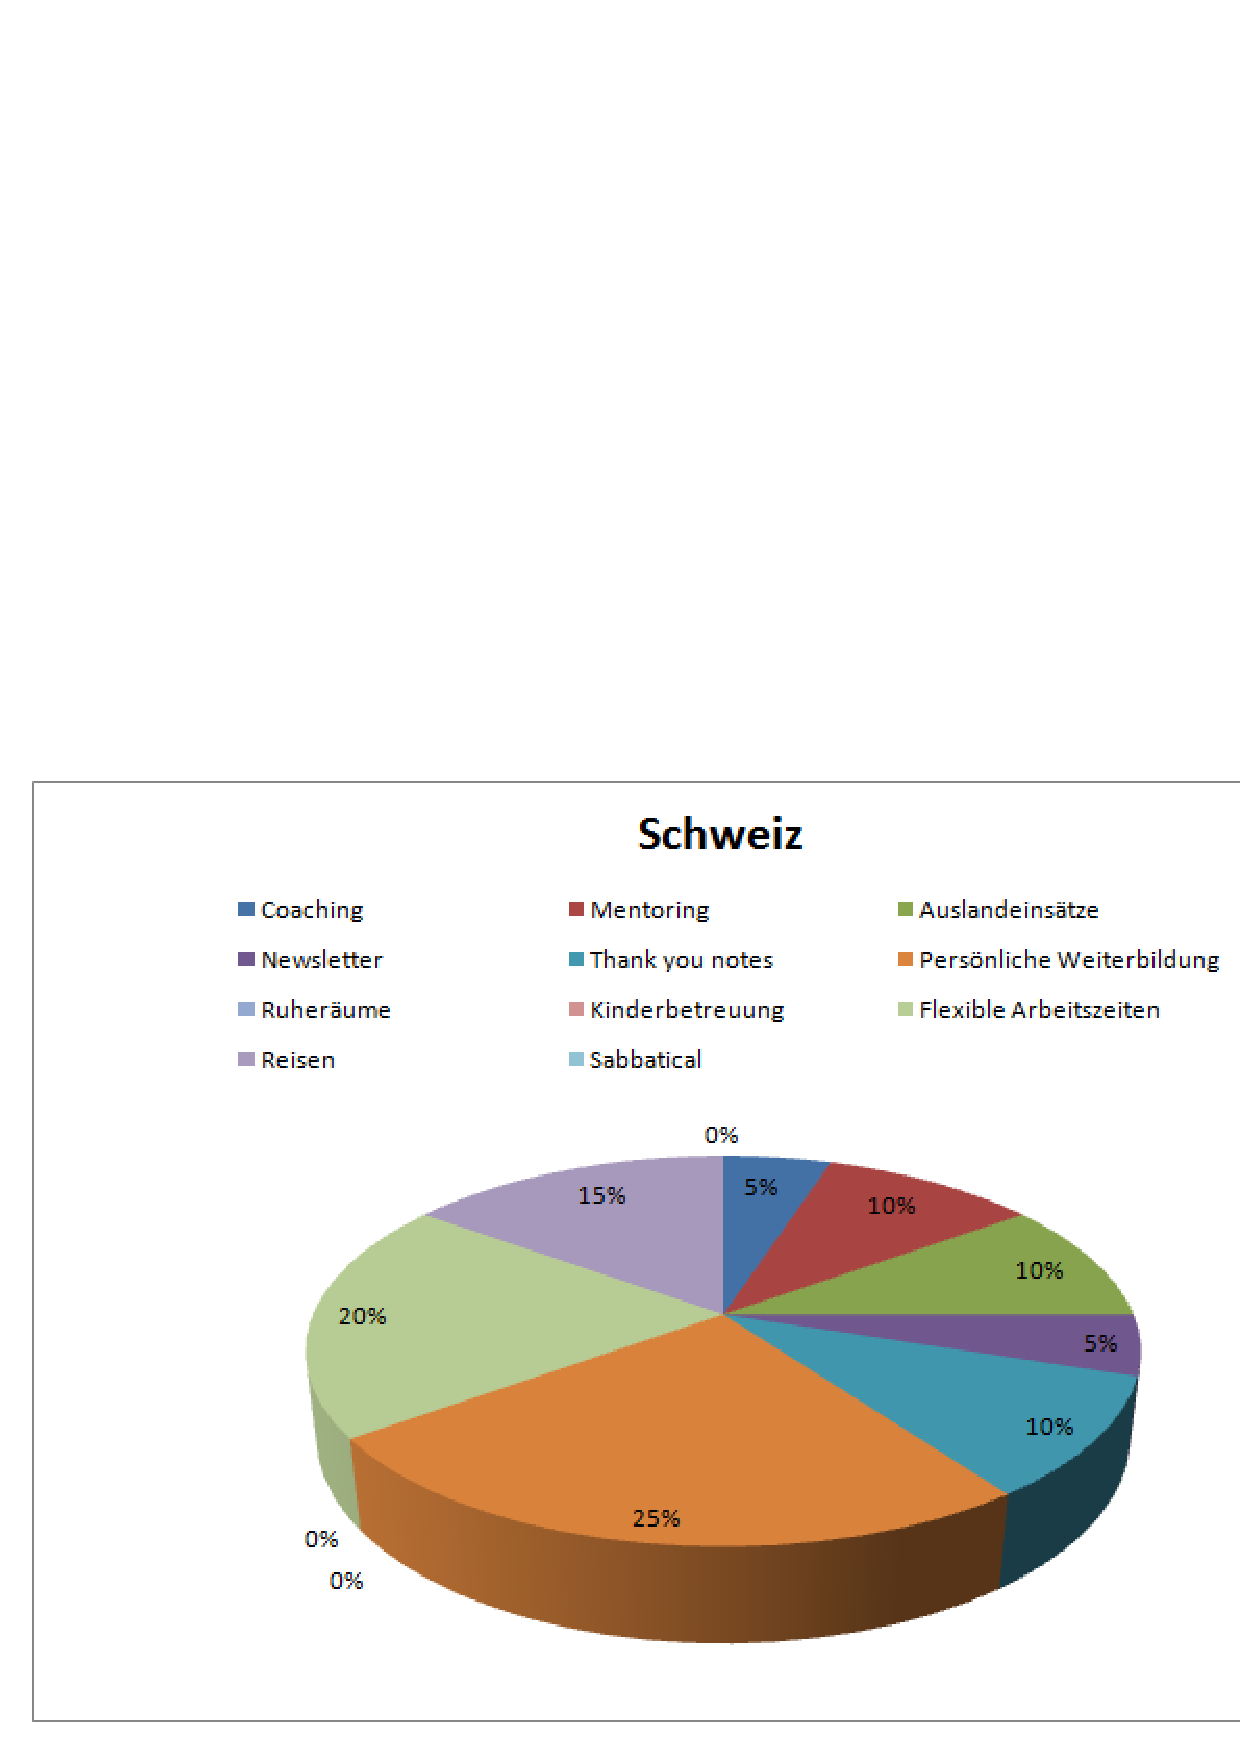
\includegraphics[width=0.9\textwidth]{chap12-unternehmen-anreiz-schweiz.png}
	\else	
		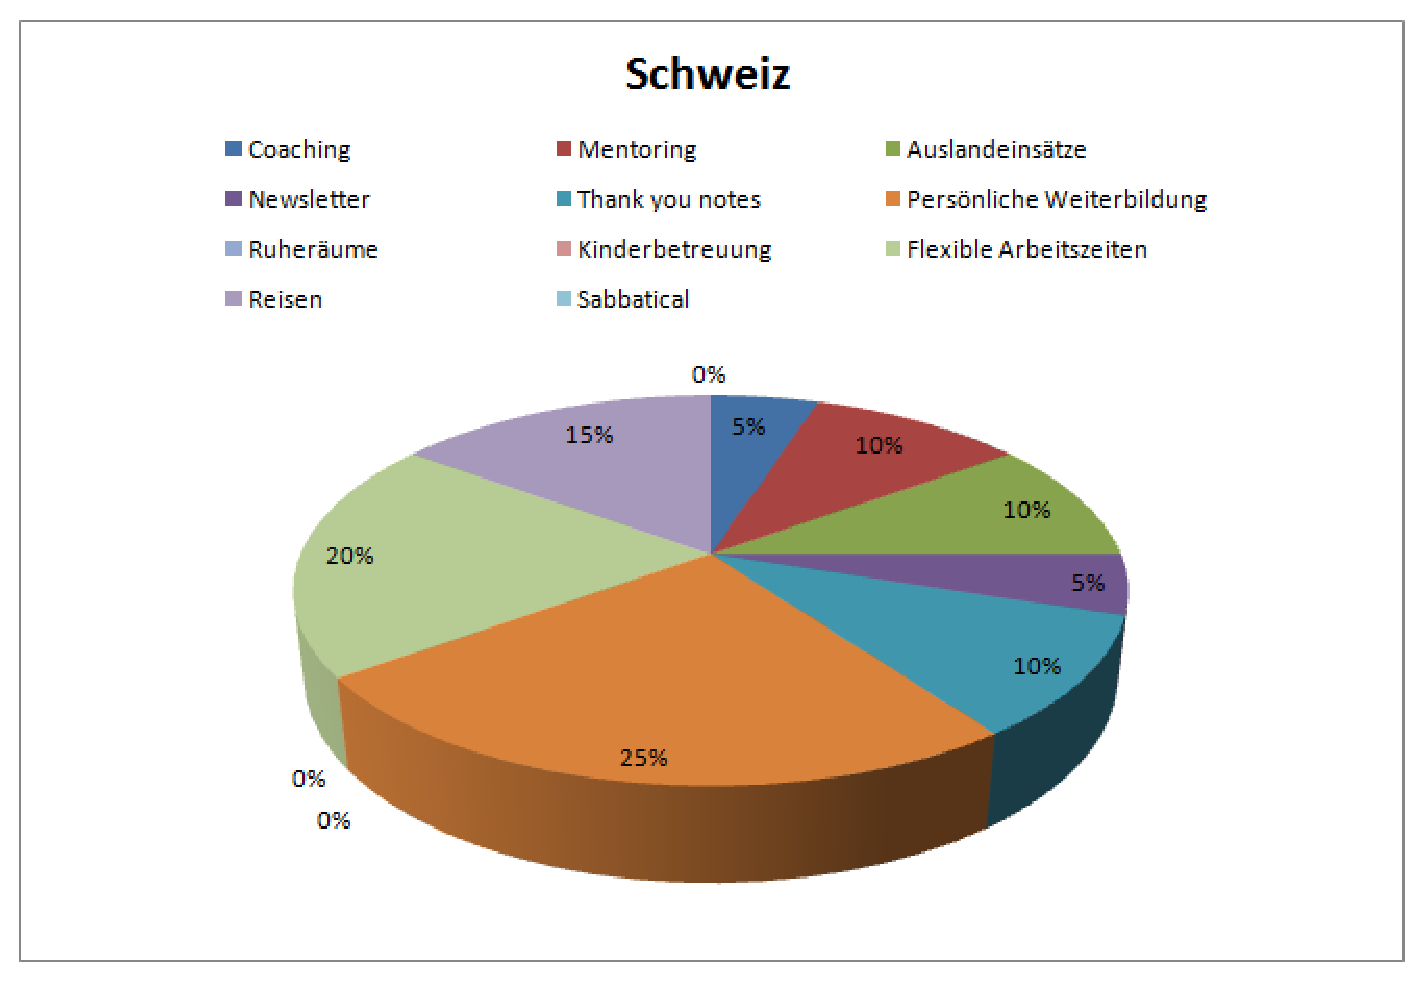
\includegraphics[width=0.9\textwidth]{chap12-unternehmen-anreiz-schweiz.eps}
	\fi
		
	\caption[Verwendete Anreize in der Schweiz]{Verwendete Anreize in der Schweiz (eigene Darstellung)}	
	\label{fig:usageInSwitzerland}
\end{figure}

\begin{figure}[h]
	\centering
		
	\ifpdf
		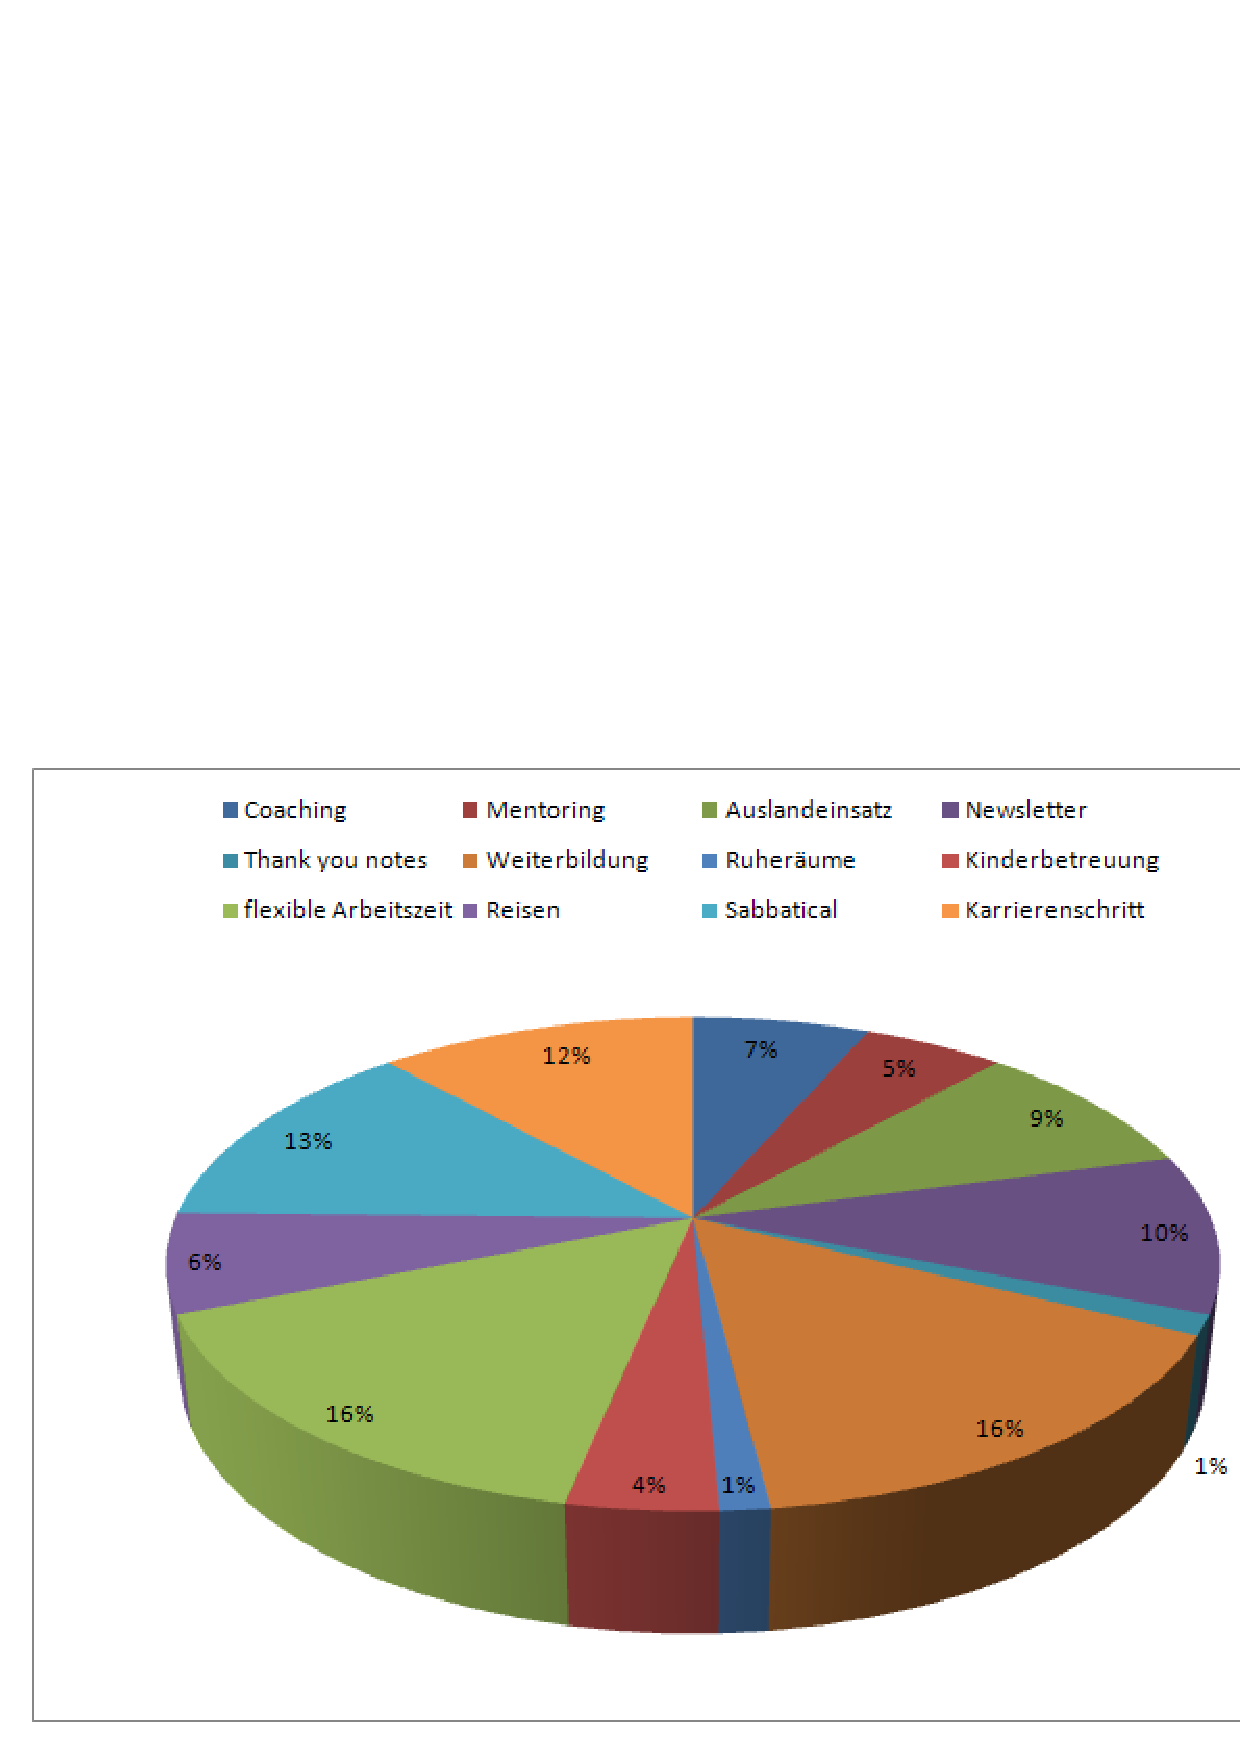
\includegraphics[width=0.9\textwidth]{chap12-mitarbeiter-beliebteAnreize.png}
	\else	
		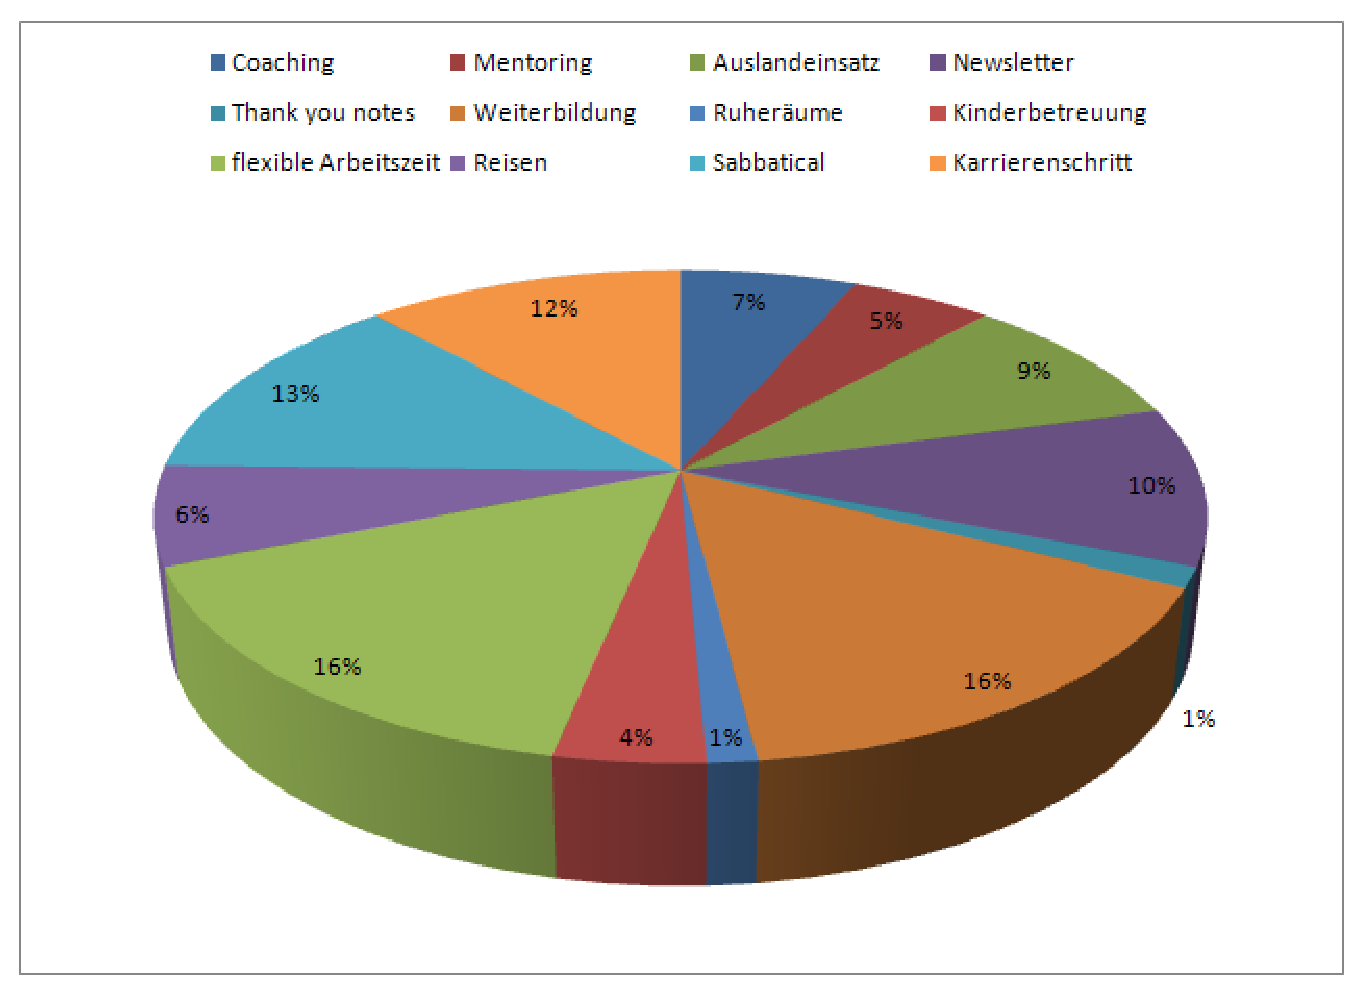
\includegraphics[width=0.9\textwidth]{chap12-mitarbeiter-beliebteAnreize.eps}
	\fi
		
	\caption[Beliebtheitsgrad von immaterielle Anreizen]{Beliebtheitsgrad von immaterielle Anreizen (eigene Darstellung)}	
	\label{fig:maImmatAnreizeFavo}
\end{figure}

\begin{figure}[h]
	\centering
		
	\ifpdf
		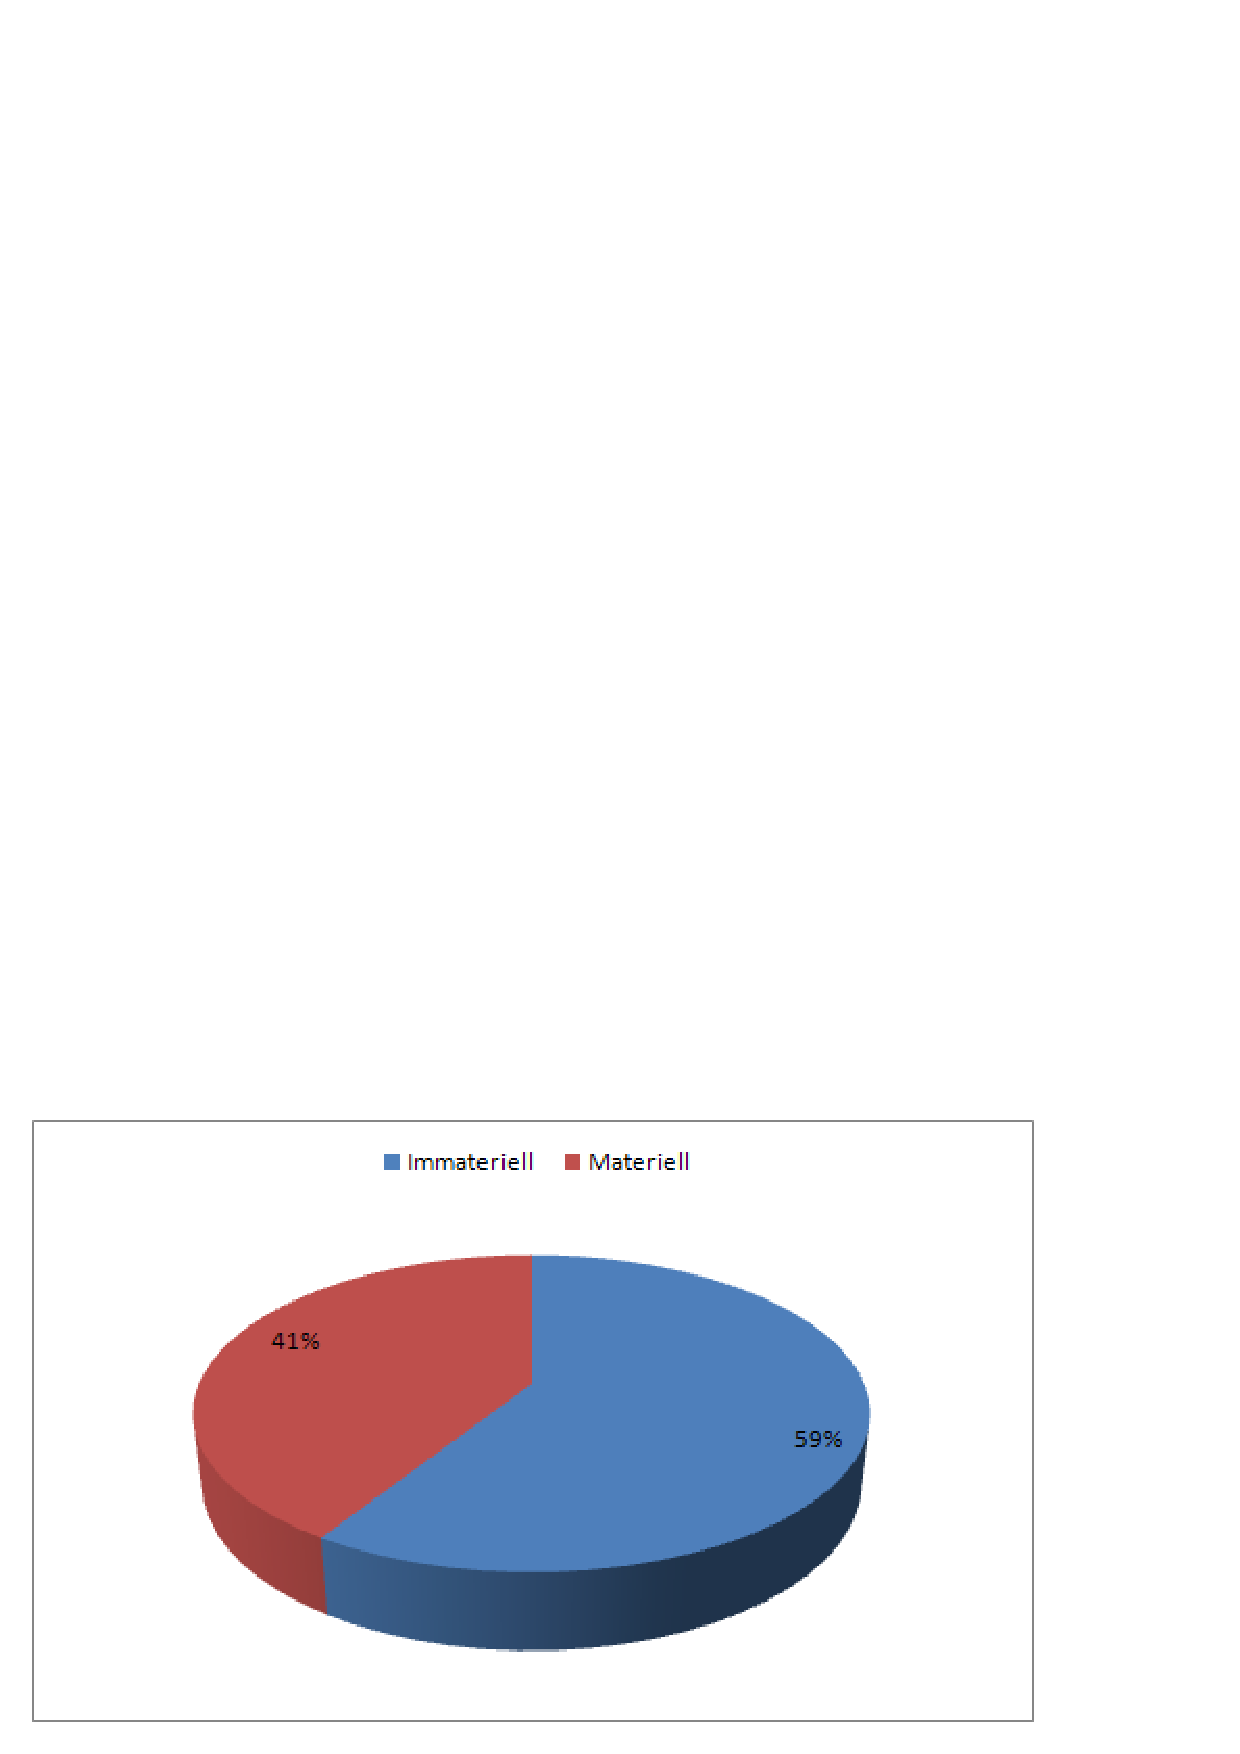
\includegraphics[width=0.9\textwidth]{chap12-mitarbeiter-anreizDiff.png}
	\else	
		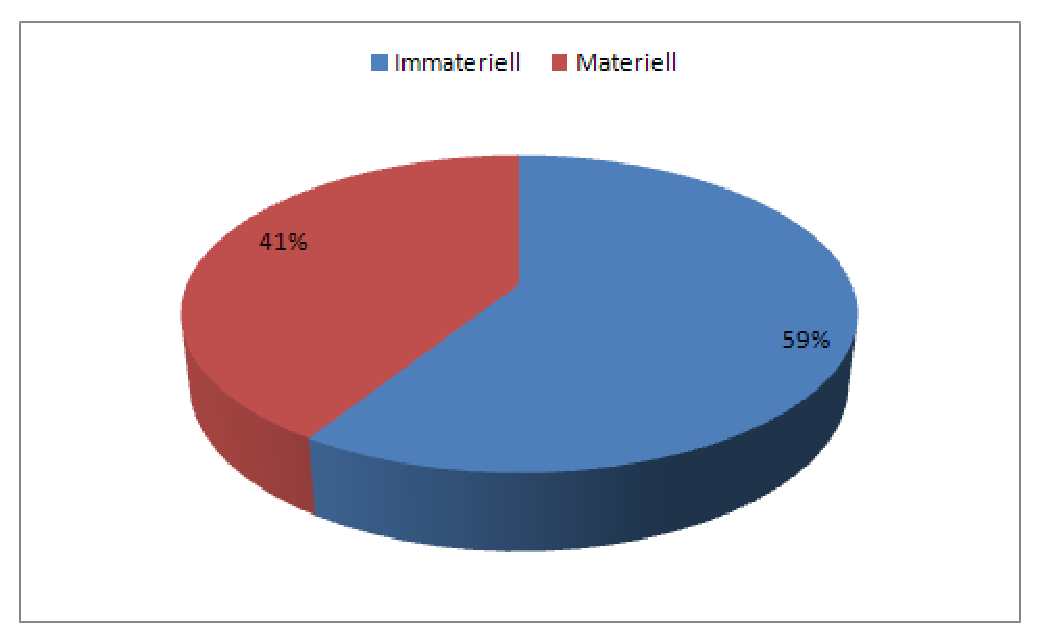
\includegraphics[width=0.9\textwidth]{chap12-mitarbeiter-anreizDiff.eps}
	\fi
		
	\caption[Anreizverh�ltnis bei den Mitarbeitern]{Anreizverh�ltnis bei den Mitarbeitern (eigene Darstellung)}	
	\label{fig:maAnreizeDiff}
\end{figure}

\begin{figure}[h]
	\centering
		
	\ifpdf
		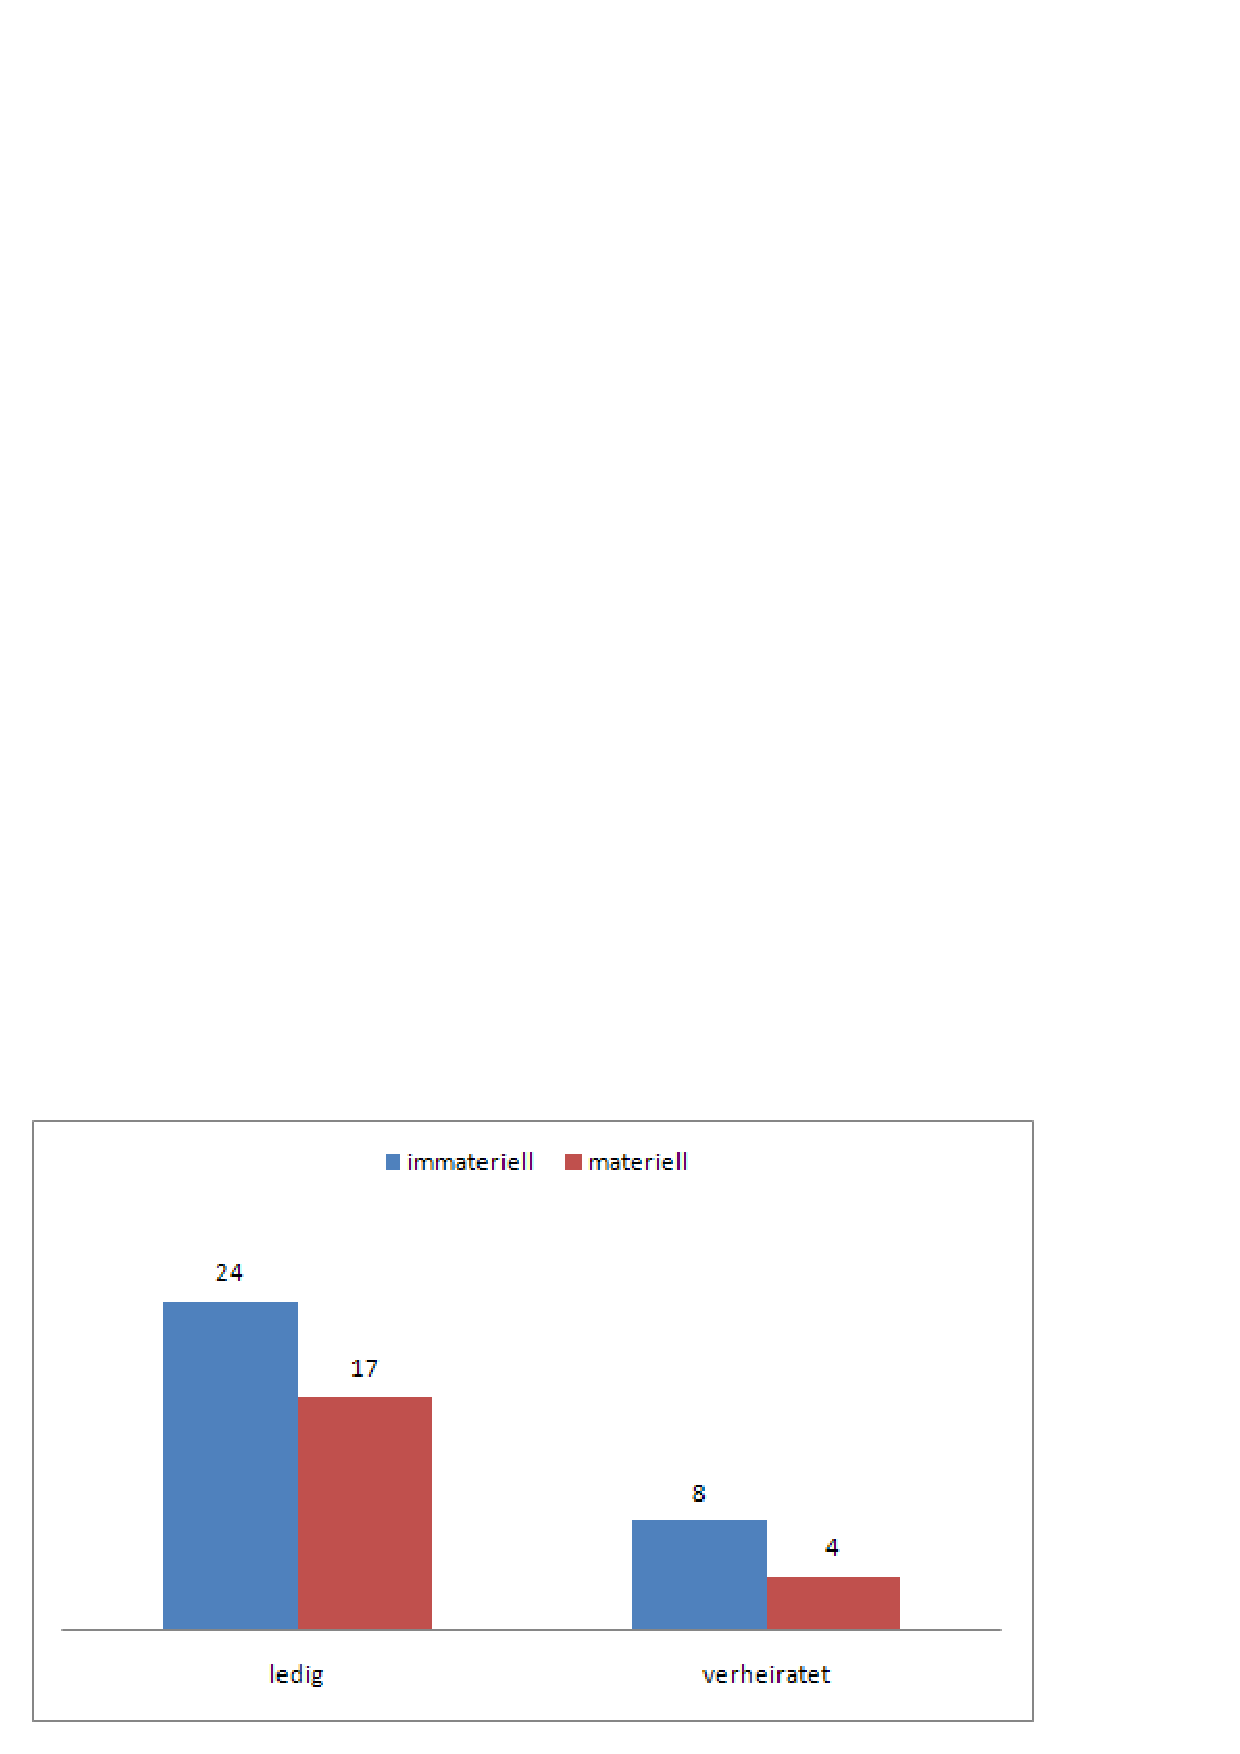
\includegraphics[width=0.9\textwidth]{chap12-mitarbeiter-beliebteAnreizeNachZivilstand.png}
	\else	
		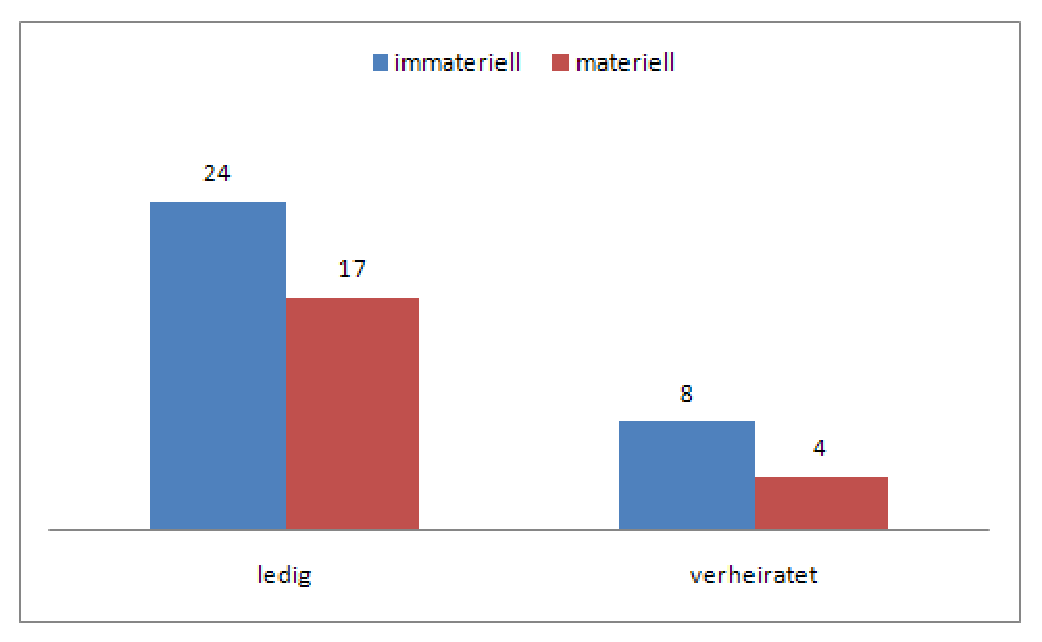
\includegraphics[width=0.9\textwidth]{chap12-mitarbeiter-beliebteAnreizeNachZivilstand.eps}
	\fi
		
	\caption[Beliebtheitsgrad von Anreizen je Zivilstand]{Beliebtheitsgrad von Anreizen je Zivilstand (eigene Darstellung)}	
	\label{fig:maAnreizeZivilstand}
\end{figure}